\documentclass[12pt,a4paper]{report}

% 1. Gọi file cấu hình
\usepackage[left=1.50cm, right=2.00cm, top=2.00cm, bottom=2.5cm, includehead, includefoot, headheight=45pt]{geometry}
\usepackage{mathpazo}
\usepackage{graphicx}
\usepackage{xcolor}
\usepackage{fontspec}
\usepackage{tabularx}
\usepackage{caption}
\usepackage{float}
\usepackage{booktabs}
\usepackage{setspace}
\usepackage{amsmath, amssymb, amsfonts}
\usepackage{array}
\usepackage{hhline}
\usepackage{algorithm}
\usepackage{algpseudocode}

%---header
\usepackage{fancyhdr}
\fancyhf{} % Xóa định dạng mặc định

% Cấu hình Header (Trên)
\fancyhead[L]{%
    \begin{minipage}[b]{0.12\textwidth}
        
\includegraphics[height=1.2cm]{images/logo-hcmus.png} 
    \end{minipage}%
    \begin{minipage}[b]{0.88\textwidth}
        \large Trường ĐH Khoa học Tự nhiên - ĐHQG HCM \\
        Khoa Công Nghệ Thông Tin
    \end{minipage}\vspace{-0.5cm}
}

% Cấu hình Footer (Dưới)
\fancyfoot[L]{Đồ án 1 | Ma trận và Tính toán Khoa học}
\fancyfoot[R]{Trang \thepage}

% Độ dày của đường gạch ngang
\renewcommand{\headrulewidth}{0.5pt} 
\renewcommand{\footrulewidth}{0.5pt} 

\setlength{\headheight}{45pt} % Tránh cảnh báo của hệ thống

% Ép các trang bắt đầu Chapter (Part) vẫn hiện Header/Footer
\makeatletter
\let\ps@plain\ps@fancy
\makeatother

\usepackage{tikz}
\usetikzlibrary{shapes.geometric, arrows}
\usepackage{tocloft}
\usepackage{multirow}
\usepackage{multicol}
\usepackage{colortbl}
\usepackage{longtable}
\usepackage{fancybox}
\usepackage{etoolbox}
% \usepackage{xeCJK} % nếu cần tiếng Việt/tiếng Á

\usepackage[hidelinks]{hyperref}

% --- Cấu hình Font chữ (Bắt buộc dùng XeLaTeX) ---
\setmonofont{Courier New} % Giúp code hiển thị đúng tiếng Việt
\setmainfont{Times New Roman} 

% --- Cấu hình Trích dẫn và Liên kết ---
\usepackage[backend=biber, style=ieee]{biblatex}
\addbibresource{references.bib}
\definecolor{fitblue}{RGB}{0, 80, 150}
\hypersetup{colorlinks=true, citecolor=blue, urlcolor=fitblue}

\makeatletter
\renewcommand{\@cite}[2]{\textcolor{blue}{[#1\if@tempswa , #2\fi]}}
\makeatother

% --- Cấu hình hiển thị Code (Python) ---
\usepackage{listings}
\definecolor{dkgreen}{rgb}{0,0.6,0}
\definecolor{mauve}{rgb}{0.58,0,0.82}

\lstset{ 
    frame=single, 
    language=Python, 
    aboveskip=3mm, 
    belowskip=3mm, 
    showstringspaces=false, 
    columns=flexible, 
    basicstyle={\normalsize\ttfamily}, 
    numbers=none, 
    keywordstyle=\color{blue}, 
    commentstyle=\color{dkgreen}, 
    stringstyle=\color{mauve}, 
    breaklines=true, 
    breakatwhitespace=true, 
    tabsize=3,
    backgroundcolor=\color{gray!10}, 
    rulecolor=\color{gray!90}
} 

\lstdefinestyle{numbered}{ 
    numbers=left, 
    numberstyle=\small\color{gray}, 
    numbersep=5pt, 
    frame=single, 
    framexleftmargin=15pt, 
    xleftmargin=15pt, 
    language=Python, 
    basicstyle={\normalsize\ttfamily},
    keywordstyle=\color{blue}, 
    commentstyle=\color{dkgreen}, 
    stringstyle=\color{mauve}, 
    breaklines=true, 
    tabsize=3
}

% --- Việt hóa các tiêu đề ---
\renewcommand{\figurename}{Hình}
\renewcommand{\tablename}{Bảng}
\renewcommand{\contentsname}{MỤC LỤC}

% --- Cấu hình Mục lục ---
\renewcommand{\cfttoctitlefont}{\LARGE\bfseries}
\setlength{\cftbeforetoctitleskip}{0pt}
\setlength{\cftaftertoctitleskip}{0pt}

% --- Định nghĩa kiểu cột tùy chỉnh ---
\newcolumntype{L}[1]{>{\raggedright\let\newline\\\arraybackslash\hspace{0pt}}m{#1}}
\newcolumntype{C}[1]{>{\centering\let\newline\\\arraybackslash\hspace{0pt}}m{#1}}
\newcolumntype{R}[1]{>{\raggedleft\let\newline\\\arraybackslash\hspace{0pt}}m{#1}}

\setlength{\parskip}{0.8em}

% --- Cấu hình Tiêu đề ---
\usepackage{titlesec}
\titleformat{\chapter}[hang]{\normalfont\LARGE\bfseries}{\thechapter}{1em}{}
\titlespacing*{\chapter}{0pt}{-10pt}{20pt} % Chỉnh khoảng cách trên/dưới tiêu đề


\begin{document}

% 2. Trang bìa
\thispagestyle{empty}
\vspace*{-1.5cm} % <--- Lệnh này kéo toàn bộ khung trang bìa dịch lên trên

\begin{center}
    \setlength{\fboxrule}{1.2pt}
    \doublebox{%
        \begin{minipage}{0.95\textwidth}
            \begin{center}
                \vspace{0.6cm}
                ĐẠI HỌC QUỐC GIA THÀNH PHỐ HỒ CHÍ MINH\\
                TRƯỜNG ĐẠI HỌC KHOA HỌC TỰ NHIÊN\\
                \textbf{KHOA CÔNG NGHỆ THÔNG TIN}\\[0.4em]
                -\hspace{0.01cm}-\hspace{0.01cm}-\hspace{0.01cm}-\hspace{0.01cm}-\hspace{0.01cm}-\textbf{oOo}-\hspace{0.01cm}-\hspace{0.01cm}-\hspace{0.01cm}-\hspace{0.01cm}-\hspace{0.01cm}-\\[2em]

                % Logo
                
\includegraphics[width=0.20\textwidth]{images/logo-hcmus.png}\\[1em]

                \textbf{\LARGE BÁO CÁO ĐỒ ÁN MÔN HỌC}\\[0.5em]
                
                \textbf{MTH00051 - Toán Ứng Dụng và Thống Kê}\\[1em]
                \textcolor{fitblue}{\LARGE{\textbf{ĐỒ ÁN 1: MA TRẬN VÀ TÍNH TOÁN KHOA HỌC}}}\\[3em]

                \begin{tabular}{ l l }
                            \textbf{Giảng viên hướng dẫn} & : ThS. Võ Nam Thục Đoan \\
                                  & \phantom{:} ThS. Lê Nhựt Nam \\ [0.5em]
                     \textbf{Nhóm sinh viên thực hiện} & : Nhóm 1
                \end{tabular}\\[1.5em]

                % Bảng thành viên
                \renewcommand{\arraystretch}{1.2}
                \begin{tabular}{ c  l  l }
                    \textbf{STT} & \textbf{MSSV} & \textbf{Họ và tên} \\
                    1 & 24120239 & Phí Công Tuấn (Nhóm Trưởng) \\
                    2 & 24120260 & Trương Tuấn Anh \\
                    3 & 24120295 & Phạm Xuân Duy \\
                    4 & 24120301 & Lâm Đông Hải \\
                    5 & 24120315 & Phạm Huy Hoàng \\
                \end{tabular}

                \vspace{4em} % <--- Đã giảm khoảng cách ở đây từ 9em xuống 4em để khung nhỏ lại
                \textbf{TP. Hồ Chí Minh, tháng 04 năm 2026}
                \vspace{1.5em} % Tạo một chút khoảng trống nhỏ ở đáy khung cho đẹp
            \end{center}
        \end{minipage}
    }
\end{center}

% 3. Cấu hình số trang và Mục lục
\newpage
\pagestyle{fancy}
\pagenumbering{arabic}
\setcounter{page}{1}
\renewcommand{\contentsname}{}        % Xóa chữ "Mục lục" mặc định
\renewcommand{\listtablename}{}       
\renewcommand{\listfigurename}{}      

\chapter*{\centering{MỤC LỤC}}
\phantomsection
\addcontentsline{toc}{chapter}{\textcolor{fitblue}{MỤC LỤC}}
{\setstretch{1.2}
\tableofcontents
\newpage
\newpage
}

%  % 4. Các  nội dung chính

\newpage
\chapter*{\centering{\MakeUppercase{Bảng phân công công việc}}}
\addcontentsline{toc}{chapter}{\textcolor{fitblue}{\MakeUppercase{Bảng phân công công việc}}}
% \begin{center}
%     \renewcommand{\arraystretch}{1.3}
%     \resizebox{\textwidth}{!}{%
%         \begin{tabular}{|c | l | l | p{9cm} | c |}
%         \hline
%         \textbf{STT} & \textbf{MSSV} & \textbf{Họ và tên} & \textbf{Nhiệm vụ} & \textbf{Đánh giá} \\
%         \hline
%         1 & 24120239 & Phí Công Tuấn & - Viết báo cáo LaTeX. \newline - Code hàm gaussian\_eliminate và back\_substitution. & 100\% \\
%         \hline
%         2 & 24120260 & Trương Tuấn Anh & - Trực quan hóa Manim (phân rã, chéo hóa). \newline - Quay và render video demo\_video.mp4 . & 100\% \\
%         \hline
%         3 & 24120295 & Phạm Xuân Duy & - Code Phần 2: Phân rã ma trận bằng thuật toán Gram-Schmidt và chéo hóa ma trận . & 100\% \\
%         \hline
%         4 & 24120301 & Lâm Đông Hải & - Trực quan hóa Manim (phân rã, chéo hóa). \newline - Quay và render video demo\_video.mp4 . & 100\% \\
%         \hline
%         5 & 24120315 & Phạm Huy Hoàng & - Code hàm determinant, inverse, rank\_and\_basis và verify\_solution. & 100\% \\
%         \hline
       
%         \end{tabular}
%     }
% \end{center}
\begin{center}
    \renewcommand{\arraystretch}{1.3}
    \resizebox{\textwidth}{!}{%
        \begin{tabular}{|c | l | l | L{9cm} | c |} % Đã đổi p{9cm} thành L{9.5cm}
        \hline
        \textbf{STT} & \textbf{MSSV} & \textbf{Họ và tên} & \textbf{Nhiệm vụ} & \textbf{Đánh giá} \\
        \hline
        1 & 24120239 & Phí Công Tuấn & - Viết báo cáo LaTeX. \newline - Code hàm gaussian\_eliminate và back\_substitution. & 100\% \\
        \hline
        2 & 24120260 & Trương Tuấn Anh & - Trực quan hóa Manim (phân rã, chéo hóa). \newline - Quay và render video demo\_video.mp4. & 100\% \\
        \hline
        3 & 24120295 & Phạm Xuân Duy & - Code Phần 2: Phân rã ma trận bằng thuật toán Gram-Schmidt và chéo hóa ma trận. & 100\% \\
        \hline
        4 & 24120301 & Lâm Đông Hải & - Trực quan hóa Manim (phân rã, chéo hóa). \newline - Quay và render video demo\_video.mp4. & 100\% \\
        \hline
        5 & 24120315 & Phạm Huy Hoàng & - Code hàm determinant, inverse, rank\_and\_basis và verify\_solution. & 100\% \\
        \hline
        \end{tabular}
    }
\end{center}
% \newpage
% \chapter*{\centering{\MakeUppercase{CHƯƠNG 1. TỔNG QUAN CHƯƠNG TRÌNH}}}
% \addcontentsline{toc}{chapter}{\textcolor{fitblue}{\MakeUppercase{CHƯƠNG 1. TỔNG QUAN CHƯƠNG TRÌNH}}}

% Nội dung chương 1 viết tại đây...\cite{cppreference}


\newpage
\chapter*{\centering{\MakeUppercase{PHẦN 1: PHÉP KHỬ GAUSS VÀ CÁC ỨNG Dụng}}}
\phantomsection
\addcontentsline{toc}{chapter}{\textcolor{fitblue}{\MakeUppercase{PHẦN 1: PHÉP KHỬ GAUSS VÀ CÁC ỨNG DỤNG}}}

Nội dung phần này tập trung vào việc tự xây dựng (from scratch) phép khử Gauss có áp dụng kỹ thuật chọn phần tử chốt (Partial Pivoting) và các ứng dụng của nó trong giải tích ma trận.

\section*{1.1. Cơ sở lý thuyết}
\phantomsection
\addcontentsline{toc}{section}{1.1. Cơ sở lý thuyết}

\subsection*{1.1.1. Phương pháp khử Gauss và Gauss-Jordan}
\phantomsection
\addcontentsline{toc}{subsection}{1.1.1. Phương pháp khử Gauss và Gauss-Jordan}


% Viết lý thuyết về ma trận tăng cường, phép biến đổi dòng sơ cấp, và dạng bậc thang (REF, RREF) vào đây.
Quá trình khử Gauss sử dụng ba phép biến đổi dòng sơ cấp:
\begin{enumerate}
    \item $R_{i} \leftrightarrow R_{j}$: Hoán đổi vị trí hai dòng $i$ và $j$.
    \item $R_{i} \leftarrow c \cdot R_{i}$ ($c \neq 0$): Nhân một dòng với một hằng số khác không.
    \item $R_{i} \leftarrow R_{i} + c \cdot R_{j}$: Cộng một bội số của dòng này vào dòng khác.
\end{enumerate}

Mục tiêu của phép khử Gauss là đưa ma trận về Dạng bậc thang dòng (Row Echelon Form - REF), trong đó các dòng toàn số 0 nằm dưới cùng và phần tử chỉ huy (pivot) của dòng dưới luôn nằm bên phải pivot của dòng trên. Phương pháp Gauss-Jordan tiến xa hơn bằng cách đưa ma trận về Dạng bậc thang dòng rút gọn (Reduced REF - RREF), yêu cầu thêm điều kiện mọi pivot phải bằng 1 và các phần tử khác trong cùng cột với pivot phải bằng 0.

\subsection*{1.1.2. Khử Gauss có chọn phần tử chốt (Partial Pivoting)}
\phantomsection
\addcontentsline{toc}{subsection}{1.1.2. Khử Gauss có chọn phần tử chốt (Partial Pivoting)}

% Giải thích vì sao cần Partial Pivoting để giảm sai số làm tròn.
Khi lập trình tính toán trên máy tính, thuật toán Gauss cơ bản dễ gặp lỗi chia cho 0 hoặc sai số làm tròn (round-off error) cực lớn nếu phần tử pivot quá nhỏ. 

Để khắc phục, ta áp dụng kỹ thuật Partial Pivoting: Tại bước khử thứ $k$, thay vì lấy luôn $a_{kk}$ làm pivot, ta tìm phần tử có giá trị tuyệt đối lớn nhất trong cột $k$ từ dòng $k$ đến dòng $n$:
$$|a_{pk}^{(k)}| = \max_{k \le i \le n} |a_{ik}^{(k)}|$$
Sau đó, hoán đổi dòng $k$ và dòng $p$ trước khi thực hiện phép khử. Điều này đảm bảo các nhân tử luôn có trị tuyệt đối $\le 1$, giúp duy trì tính ổn định số học.
\subsection*{1.1.3. Tính định thức, ma trận nghịch đảo và hạng ma trận}
\phantomsection
\addcontentsline{toc}{subsection}{1.1.3. Tính định thức, ma trận nghịch đảo và hạng ma trận}

% Trình bày công thức tính Det qua ma trận tam giác trên, cách tìm A^-1 bằng [A|I], và cách xác định Rank.
\textbf{Tính định thức:} Khi đưa ma trận vuông $A$ về ma trận tam giác trên $U$ bằng phép khử Gauss, định thức của $A$ bằng tích các phần tử trên đường chéo chính của $U$, nhân với $(-1)^s$, trong đó $s$ là số lần hoán đổi dòng đã thực hiện:
$$det(A) = (-1)^{s} \cdot \prod_{i=1}^{n} u_{ii}$$

\textbf{Tìm ma trận nghịch đảo:} Một ma trận vuông $A$ khả nghịch khi $det(A) \neq 0$. Bằng phương pháp Gauss-Jordan, ta lập ma trận tăng cường ghép với ma trận đơn vị $[A|I_n]$. Khi thực hiện biến đổi sơ cấp đưa vế trái về dạng RREF, vế phải sẽ trở thành ma trận nghịch đảo $A^{-1}$: $[A|I_n] \xrightarrow{\text{Gauss-Jordan}} [I_n|A^{-1}]$.

\textbf{Hạng và Cơ sở không gian:}
Hạng (rank) của ma trận $A$ chính là số dòng khác $0$ trong dạng REF của nó (hoặc số pivot). 
\begin{itemize}
    \item \textbf{Cơ sở không gian cột ($\mathcal{C}(A)$):} Tập hợp các cột của ma trận $A$ ban đầu tương ứng với các cột chứa pivot.
    \item \textbf{Cơ sở không gian dòng ($\mathcal{R}(A)$):} Tập hợp các dòng khác $0$ trong ma trận REF.
    \item \textbf{Cơ sở không gian nghiệm ($\mathcal{N}(A)$):} Tập nghiệm cơ bản của hệ phương trình thuần nhất $Ax = 0$.
\end{itemize}

\section*{1.2. Phân tích thuật toán}
\phantomsection
\addcontentsline{toc}{section}{1.2. Phân tích thuật toán}
% Viết mã giả (Pseudocode) hoặc lưu đồ thuật toán tại đây.
Dưới đây là mô tả chi tiết các bước thực thi của Thuật toán khử Gauss có Partial Pivoting để giải hệ $Ax = b$:
\\
\textbf{Đầu vào:} Ma trận $A \in \mathbb{R}^{n \times m}$, vector $b \in \mathbb{R}^{n}$.\\
\textbf{Đầu ra:} Nghiệm $x$, số lần hoán đổi dòng $s$.

\textbf{Bước 1: Khởi tạo}\\
Tạo ma trận tăng cường $M = [A|b]$ và đặt biến đếm số lần hoán đổi $s = 0$.

\textbf{Bước 2: Quá trình khử tiến (Forward Elimination)}\\
Lặp $k$ từ $1$ đến $n$:
\begin{itemize}
    \item \textit{Tìm Pivot:} Tìm chỉ số dòng $p$ ($p \ge k$) sao cho $|M_{pk}|$ đạt giá trị lớn nhất. Nếu $|M_{pk}| < \epsilon$ (với $\epsilon$ rất nhỏ), cảnh báo ma trận suy biến.
    \item \textit{Hoán đổi dòng:} Nếu $p \neq k$, thực hiện hoán đổi dòng $k \leftrightarrow p$ và tăng $s = s + 1$.
    \item \textit{Khử các dòng dưới:} Lặp $i$ từ $k+1$ đến $n$. Tính nhân tử $l_{ik} = \frac{M_{ik}}{M_{kk}}$. Cập nhật dòng $i$: $M_{i} \leftarrow M_{i} - l_{ik} \cdot M_{k}$.
\end{itemize}

\textbf{Bước 3: Quá trình thế ngược (Back Substitution)}\\
Giải hệ tam giác trên từ dưới lên trên. Lặp $i$ từ $n$ lùi về $1$:
$$x_{i} = \frac{1}{M_{ii}} \left( M_{i, m+1} - \sum_{j=i+1}^{n} M_{ij}x_{j} \right)$$
\section*{1.3. Cài đặt Python và Kiểm chứng}
\phantomsection
\addcontentsline{toc}{section}{1.3. Cài đặt Python và Kiểm chứng}

Trong phần này, nhóm sẽ trình bày mã nguồn cài đặt và các test case để chứng minh tính đúng đắn của thuật toán, có đối chiếu với thư viện NumPy.

\subsection*{1.3.1. Cài đặt phép khử Gauss và Partial Pivoting}
\phantomsection
\addcontentsline{toc}{subsection}{1.3.1. Cài đặt phép khử Gauss và Partial Pivoting}
Đoạn code sau cài đặt hàm \texttt{gaussian\_eliminate(A, b)} - Trả về ma trận sau khi khử, nghiệm x, số lần hoán đổi:

\begin{algorithm}[H]
\caption{Khử Gauss với Partial Pivoting (Chọn phần tử chốt một phần)}
\label{alg:gaussian_elimination}
\begin{algorithmic}[1]
\Procedure{GAUSSIAN\_ELIMINATE}{$A, b, verbose$}
    \State $m \gets$ Số hàng của $A$
    \State $n \gets$ Số cột của $A$
    \State Khởi tạo số lần hoán đổi $s \gets 0$, dung sai $\epsilon \gets 10^{-12}$
    
    \State Tạo ma trận tăng cường $M \gets [A | b]$ \Comment{Kích thước $m \times (n+1)$}
    \State $r \gets 0$ \Comment{Chỉ số hàng pivot hiện tại}
    
    \For{$j \gets 0$ to $n-1$} \Comment{Duyệt qua từng cột}
        \If{$r \geq m$} 
            \State \textbf{break} \Comment{Đã xét hết các hàng}
        \EndIf
        
        \State Tìm $p \in [r, m-1]$ sao cho $|M[p][j]| = \max_{r \leq i < m} |M[i][j]|$
        \State $max\_val \gets |M[p][j]|$
        
        \If{$max\_val < \epsilon$}
            \State \textbf{continue} \Comment{Không có pivot, chuyển sang cột tiếp theo}
        \EndIf
        
        \If{$p \neq r$}
            \State Hoán đổi hàng $r$ và hàng $p$ của $M$: $M[r] \leftrightarrow M[p]$
            \State $s \gets $ $s + 1$
        \EndIf
        
        \For{$i \gets r+1$ to $m-1$} \Comment{Khử các phần tử dưới pivot}
            \State $factor \gets M[i][j] / M[r][j]$
            \State $M[i][j] \gets 0$ \Comment{Gán bằng 0 để tránh sai số làm tròn}
            \For{$k \gets j+1$ to $n$} \Comment{Khử đến cột cuối cùng (gồm cả $b$)}
                \State $M[i][k] \gets M[i][k] - factor \times M[r][k]$
            \EndFor
        \EndFor
        
        \State $r \gets r + 1$ \Comment{Chuyển sang hàng pivot tiếp theo}
    \EndFor
    
    \State Tách ma trận tam giác trên $U$ và vector $c$ từ ma trận tăng cường $M$
    \State $x \gets$ \Call{BACK\_SUBSTITUTION}{$U, c$} \Comment{Gọi hàm thế ngược}
    
    \If{$verbose = \text{True}$ \textbf{and} $x$ có vô số nghiệm}
        \State In công thức tổng quát của hệ phương trình
    \EndIf
    
    \State \Return $(M, x, s)$
\EndProcedure
\end{algorithmic}
\end{algorithm}

Đoạn code sau cài đặt hàm \texttt{back\_substitution(U, c)} -  Giải hệ tam giác trên:

% ==========================================
% THUẬT TOÁN THẾ NGƯỢC - PHẦN 1
% ==========================================
\begin{algorithm}[H]
\caption{Quá trình Thế ngược (Back Substitution) - Phần 1: Tiền xử lý}
\label{alg:back_substitution_1}
\begin{algorithmic}[1]
\Procedure{BACK\_SUBSTITUTION}{$U, c$}
    \State $m, n \gets$ Kích thước của ma trận tam giác trên $U$
    \State Dung sai $\epsilon \gets 10^{-12}$
    \State Khởi tạo danh sách hàng chốt $R_{piv} \gets \emptyset$, cột chốt $C_{piv} \gets \emptyset$
    
    \State \Comment{\textbf{Bước 1: Xác định vị trí các phần tử chốt}}
    \State $r \gets 0$
    \For{$j \gets 0$ to $n-1$}
        \If{$r < m$ \textbf{and} $|U[r][j]| > \epsilon$}
            \State Thêm $r$ vào $R_{piv}$, thêm $j$ vào $C_{piv}$
            \State $r \gets r + 1$
        \EndIf
    \EndFor
    
    \State \Comment{\textbf{Bước 2: Kiểm tra tính có nghiệm của hệ}}
    \For{$i \gets r$ to $m-1$} \Comment{Xét các dòng toàn số 0 của $U$}
        \If{$|c[i]| > \epsilon$}
            \State \Return "Hệ phương trình vô nghiệm"
        \EndIf
    \EndFor
    
    \State \Comment{\textbf{Bước 3: Xác định biến tự do và Khởi tạo ma trận nghiệm}}
    \State Tập các cột tự do $F \gets \{0, 1, \dots, n-1\} \setminus C_{piv}$
    \State $k_{free} \gets |F|$ \Comment{Số lượng biến tự do}
    \State Khởi tạo ma trận hệ số $X_{coef}$ kích thước $n \times (1 + k_{free})$ với các phần tử $0$
    
    \For{mỗi chỉ số $idx$ và cột $f_j \in F$}
        \State $X_{coef}[f_j][1 + idx] \gets 1.0$ \Comment{Gán hệ số 1 cho chính biến tự do đó}
    \EndFor
    
    \State \Comment{\textit{-- Thuật toán tiếp tục ở trang sau --}}
\EndProcedure
\end{algorithmic}
\end{algorithm}

\newpage % <--- Lệnh ép sang trang mới để tránh đè footer

% ==========================================
% THUẬT TOÁN THẾ NGƯỢC - PHẦN 2
% ==========================================
\begin{algorithm}[H]
\caption{Quá trình Thế ngược (Back Substitution) - Phần 2: Giải nghiệm}
\label{alg:back_substitution_2}
\begin{algorithmic}[1]
\Procedure{BACK\_SUBSTITUTION}{$U, c$} \Comment{\textit{Tiếp tục từ Phần 1}}
    
    \State \Comment{\textbf{Bước 4: Thế ngược từ dưới lên trên}}
    \For{$i \gets |C_{piv}| - 1$ \textbf{downto} $0$}
        \State $pc \gets C_{piv}[i]$, $pr \gets R_{piv}[i]$
        \State Khởi tạo mảng $coef$ kích thước $(1 + k_{free})$ với các phần tử $0$
        \State $coef[0] \gets c[pr]$ \Comment{Gán hằng số ban đầu}
        
        \For{$j \gets pc + 1$ to $n-1$}
            \If{$|U[pr][j]| > \epsilon$}
                \For{$k \gets 0$ to $k_{free}$}
                    \State $coef[k] \gets coef[k] - U[pr][j] \times X_{coef}[j][k]$
                \EndFor
            \EndIf
        \EndFor
        
        \State $piv \gets U[pr][pc]$
        \State $X_{coef}[pc] \gets coef / piv$ \Comment{Lưu hệ số tham số của biến chốt}
    \EndFor
    
    \State \Comment{\textbf{Bước 5: Trả về kết quả}}
    \If{$k_{free} = 0$}
        \State \Return $X_{coef}[:][0]$ \Comment{Nghiệm duy nhất (chỉ lấy cột hằng số)}
    \Else
        \State \Return $(X_{coef}, F)$ \Comment{Vô số nghiệm (trả về ma trận tham số)}
    \EndIf
\EndProcedure
\end{algorithmic}
\end{algorithm}

\subsection*{1.3.2. Tính định thức và Ma trận nghịch đảo}
\phantomsection
\addcontentsline{toc}{subsection}{1.3.2. Tính định thức và Ma trận nghịch đảo}

Đoạn code sau cài đặt hàm \texttt{determinant(A)} - Tính det(A) qua khử Gauss.
% \begin{lstlisting}[style=numbered, language=Python]
% def determinant(A):
%     """
%     Tính định thức det(A) qua phép khử Gauss.
%     Công thức: det(A) = (-1)^s * tích các phần tử đường chéo của U.

%     Parameters:
%     - A: Ma trận vuông (list of lists), kích thước n x n.

%     Returns:
%     - float: Giá trị định thức.
%     """
%     n = len(A)
%     if any(len(row) != n for row in A):
%         raise ValueError("Định thức chỉ xác định cho ma trận vuông.")

%     b_dummy = [0.0] * n
%     try:
%         # verbose=False: tránh in nghiệm thừa khi gọi nội bộ
%         M_aug, _, s = gaussian_eliminate(A, b_dummy, verbose=False)

%         # det = (-1)^s * tích đường chéo chính của U
%         det = (-1.0) ** s
%         for i in range(n):
%             det *= M_aug[i][i]

%         # Làm sạch kết quả gần 0 (tránh -0.0 hoặc 1e-15)
%         return 0.0 if abs(det) < 1e-12 else det
%     except:
%         return 0.0
% \end{lstlisting}

\begin{algorithm}[H]
\caption{Tính định thức của ma trận qua phép khử Gauss}
\label{alg:determinant}
\begin{algorithmic}[1]
\Procedure{DETERMINANT}{$A$}
    \State $n \gets$ Số lượng hàng của ma trận $A$
    
    \If{Có bất kỳ hàng nào của $A$ có độ dài khác $n$}
        \State \textbf{raise} Lỗi "Định thức chỉ xác định cho ma trận vuông."
    \EndIf
    
    \State Khởi tạo mảng $b\_dummy \gets [0.0, 0.0, \dots, 0.0]$ gồm $n$ phần tử
    
    \State \textbf{try:}
        \State $(M_{aug}, \_, s) \gets$ \Call{GAUSSIAN\_ELIMINATE}{$A, b\_dummy, \text{False}$}
        \State $det \gets (-1)^s$ \Comment{Dấu phụ thuộc vào số lần hoán đổi dòng $s$}
        
        \For{$i \gets 0$ to $n-1$}
            \State $det \gets det \times M_{aug}[i][i]$ \Comment{Tích các phần tử trên đường chéo}
        \EndFor
        
        \If{$|det| < 10^{-12}$}
            \State \Return $0.0$ \Comment{Tránh sai số cực nhỏ hoặc $-0.0$}
        \Else
            \State \Return $det$
        \EndIf
        
    \State \textbf{except:} \Comment{Bắt lỗi nếu ma trận suy biến không thể khử}
        \State \Return $0.0$
\EndProcedure
\end{algorithmic}
\end{algorithm}

Đoạn code sau cài đặt hàm \texttt{inverse(A)} - Tính $A^{-1}$ bằng phương pháp Gauss–Jordan.
% \begin{lstlisting}[style=numbered, language=Python]
% def inverse(A):
%     """
%     Tính ma trận nghịch đảo A^-1 bằng phương pháp Gauss–Jordan.
%     Biến đổi ma trận ghép [A | I] cho đến khi đạt dạng [I | A^-1].

%     Parameters:
%     - A: Ma trận vuông (list of lists), kích thước n x n.

%     Returns:
%     - list of lists: Ma trận nghịch đảo A^-1.
%     - str          : Thông báo nếu ma trận không khả nghịch.
%     """
%     n = len(A)
%     if any(len(row) != n for row in A):
%         raise ValueError("Chỉ ma trận vuông mới có khả năng nghịch đảo.")

%     # Bước 1: Tạo ma trận ghép [A | I]
%     I = [[1.0 if i == j else 0.0 for j in range(n)] for i in range(n)]
%     M = [A[i][:] + I[i][:] for i in range(n)]

%     # Bước 2: Phép khử Gauss–Jordan
%     for k in range(n):
%         # a. Chọn phần tử chốt (Partial Pivoting)
%         max_idx = k
%         for i in range(k + 1, n):
%             if abs(M[i][k]) > abs(M[max_idx][k]):
%                 max_idx = i

%         # b. Kiểm tra điều kiện tồn tại pivot
%         if abs(M[max_idx][k]) < 1e-12:
%             return f"Thông báo: Không có pivot tại cột {k+1}. Ma trận không khả nghịch."

%         # Hoán đổi dòng
%         M[k], M[max_idx] = M[max_idx], M[k]

%         # c. Chuẩn hóa dòng k: đưa pivot về 1
%         pivot = M[k][k]
%         M[k]  = [x / pivot for x in M[k]]

%         # d. Khử tất cả phần tử khác trên cột k về 0 (cả trên và dưới)
%         for i in range(n):
%             if i != k:
%                 factor  = M[i][k]
%                 M[i][k] = 0.0  # tránh sai số làm tròn nhỏ
%                 for j in range(k + 1, 2 * n):
%                     M[i][j] -= factor * M[k][j]

%     # Bước 3: Tách ma trận nghịch đảo từ nửa phải
%     return [row[n:] for row in M]
% \end{lstlisting}
% --- Vẽ tiêu đề và đường kẻ trên cùng thủ công ---


\begin{algorithm}[H]
\caption{Tính ma trận nghịch đảo bằng phương pháp Gauss-Jordan}
\label{alg:inverse}
\begin{algorithmic}[1]
\Procedure{INVERSE}{$A$}
    \State $n \gets$ Số lượng hàng của ma trận $A$
    
    \If{Có bất kỳ hàng nào của $A$ có độ dài khác $n$}
        \State \textbf{raise} Lỗi "Chỉ ma trận vuông mới có khả năng nghịch đảo."
    \EndIf
    
    \State \Comment{\textbf{Bước 1: Tạo ma trận ghép $[A | I]$}}
    \State Khởi tạo ma trận đơn vị $I$ kích thước $n \times n$
    \State Tạo ma trận tăng cường $M \gets [A | I]$ \Comment{Kích thước $n \times 2n$}
    
    \State \Comment{\textbf{Bước 2: Phép khử Gauss-Jordan}}
    \For{$k \gets 0$ to $n-1$}
        
        \State \Comment{a. Chọn phần tử chốt (Partial Pivoting)}
        \State $max\_idx \gets k$
        \For{$i \gets k+1$ to $n-1$}
            \If{$|M[i][k]| > |M[max\_idx][k]|$}
                \State $max\_idx \gets i$
            \EndIf
        \EndFor
        
        \State \Comment{b. Kiểm tra điều kiện tồn tại pivot}
        \If{$|M[max\_idx][k]| < 10^{-12}$}
            \State \Return "Thông báo: Không có pivot tại cột $k+1$. Ma trận không khả nghịch."
        \EndIf
        
        \State Hoán đổi hàng $k$ và hàng $max\_idx$ của $M$: $M[k] \leftrightarrow M[max\_idx]$
        
        \State \Comment{c. Chuẩn hóa dòng $k$: đưa phần tử chốt về 1}
        \State $piv \gets M[k][k]$
        \For{$j \gets k$ to $2n-1$}
            \State $M[k][j] \gets M[k][j] / piv$
        \EndFor
        
        \State \Comment{d. Khử tất cả phần tử khác trên cột $k$ về 0 (cả trên và dưới)}
        \For{$i \gets 0$ to $n-1$}
            \If{$i \neq k$}
                \State $factor \gets M[i][k]$
                \State $M[i][k] \gets 0$ \Comment{Tránh sai số làm tròn nhỏ}
                \For{$j \gets k+1$ to $2n-1$}
                    \State $M[i][j] \gets M[i][j] - factor \times M[k][j]$
                \EndFor
            \EndIf
        \EndFor
    \EndFor
    
    \State \Comment{\textbf{Bước 3: Tách ma trận nghịch đảo từ nửa phải}}
    \State Trích xuất các cột từ $n$ đến $2n-1$ của $M$ vào ma trận $A^{-1}$
    \State \Return $A^{-1}$
\EndProcedure
\end{algorithmic}
\end{algorithm}

\subsection*{1.3.3. Xác định Hạng và Cơ sở}
\phantomsection
\addcontentsline{toc}{subsection}{1.3.3. Xác định Hạng và Cơ sở}
% \begin{lstlisting}[style=numbered, language=Python]
% # Dán code hàm rank_and_basis(A)
% def rank_and_basis(A):
%     """
%     Tính hạng và cơ sở của ba không gian con của ma trận A:
%     - Không gian cột  C(A): sinh bởi các cột pivot của A gốc.
%     - Không gian dòng R(A): sinh bởi các dòng khác 0 trong REF.
%     - Không gian nghiệm N(A): tập nghiệm của Ax = 0.

%     Parameters:
%     - A: Ma trận (list of lists), kích thước m x n.

%     Returns:
%     - rank      : Hạng của A (int).
%     - col_basis : Cơ sở không gian cột (list of lists).
%     - row_basis : Cơ sở không gian dòng (list of lists).
%     - null_basis: Cơ sở không gian nghiệm (list of lists).
%                   Rỗng nếu A có hạng đầy đủ theo cột.
%     """
%     m, n = len(A), len(A[0])
%     eps  = 1e-12

%     # Bước 1: Đưa A về dạng REF
%     # verbose=False: tránh in nghiệm khi gọi nội bộ
%     M_aug, _, _ = gaussian_eliminate(A, [0.0] * m, verbose=False)
%     U = [row[:n] for row in M_aug]  # chỉ lấy phần ma trận, bỏ cột b

%     # Bước 2: Xác định cột pivot và hạng
%     pivot_cols = []
%     r = 0
%     for j in range(n):
%         if r < m and abs(U[r][j]) > eps:
%             pivot_cols.append(j)
%             r += 1
%     rank = len(pivot_cols)

%     # Bước 3: Cơ sở không gian dòng — các dòng khác 0 của REF
%     row_basis = [U[i][:] for i in range(rank)]

%     # Bước 4: Cơ sở không gian cột — cột pivot trên ma trận GỐC A
%     col_basis = [[A[i][j] for i in range(m)] for j in pivot_cols]

%     # Bước 5: Cơ sở không gian nghiệm (Null Space)
%     # Với mỗi biến tự do free_j: gán x[free_j]=1, biến tự do khác=0,
%     # rồi thế ngược trên U (b=0) để tìm biến pivot tương ứng.
%     free_cols  = [j for j in range(n) if j not in pivot_cols]
%     null_basis = []

%     for fj in free_cols:
%         x     = [0.0] * n
%         x[fj] = 1.0
%         for i in range(rank - 1, -1, -1):
%             pc    = pivot_cols[i]
%             val   = sum(U[i][j] * x[j] for j in range(pc + 1, n))
%             x[pc] = -val / U[i][pc]  # b = 0 nên không có số hạng tự do
%         null_basis.append(x)

%     return rank, col_basis, row_basis, null_basis
% \end{lstlisting}
% --- Vẽ tiêu đề và đường kẻ trên cùng thủ công ---


\begin{algorithm}[H]
\caption{Xác định Hạng và Cơ sở của ma trận}
\label{alg:rank_and_basis}
\begin{algorithmic}[1]
\Procedure{RANK\_AND\_BASIS}{$A$}
    \State $m, n \gets$ Kích thước của ma trận $A$
    \State Dung sai $\epsilon \gets 10^{-12}$

    \State \Comment{\textbf{Bước 1: Đưa ma trận $A$ về dạng Bậc thang (REF)}}
    \State Tạo vector $b\_zero \gets [0.0, 0.0, \dots, 0.0]$ gồm $m$ phần tử
    \State $(M_{aug}, \_, \_) \gets$ \Call{GAUSSIAN\_ELIMINATE}{$A, b\_zero, \text{False}$}
    \State Trích xuất ma trận $U$ bằng cách bỏ đi cột cuối cùng ($b$) của $M_{aug}$

    \State \Comment{\textbf{Bước 2: Xác định cột pivot và hạng}}
    \State Khởi tạo danh sách các cột chốt $pivot\_cols \gets \emptyset$
    \State $r \gets 0$
    \For{$j \gets 0$ to $n-1$}
        \If{$r < m$ \textbf{and} $|U[r][j]| > \epsilon$}
            \State Thêm $j$ vào $pivot\_cols$
            \State $r \gets r + 1$
        \EndIf
    \EndFor
    \State $rank \gets |pivot\_cols|$ \Comment{Số lượng cột chốt chính là hạng của ma trận}

    \State \Comment{\textbf{Bước 3: Xác định cơ sở không gian dòng $\mathcal{R}(A)$}}
    \State $row\_basis \gets$ $rank$ dòng đầu tiên của ma trận $U$

    \State \Comment{\textbf{Bước 4: Xác định cơ sở không gian cột $\mathcal{C}(A)$}}
    \State $col\_basis \gets$ Lấy các cột từ ma trận \textbf{GỐC} $A$ dựa trên các chỉ số trong $pivot\_cols$

    \State \Comment{\textbf{Bước 5: Xác định cơ sở không gian nghiệm $\mathcal{N}(A)$}}
    \State Tập các cột tự do $free\_cols \gets \{0, 1, \dots, n-1\} \setminus pivot\_cols$
    \State Khởi tạo danh sách cơ sở nghiệm $null\_basis \gets \emptyset$

    \For{mỗi chỉ số $f_j \in free\_cols$}
        \State Khởi tạo vector $x \gets [0.0, \dots, 0.0]$ gồm $n$ phần tử
        \State $x[f_j] \gets 1.0$ \Comment{Gán giá trị 1 cho biến tự do đang xét}
        
        \For{$i \gets rank - 1$ \textbf{downto} $0$}
            \State $pc \gets pivot\_cols[i]$
            \State $val \gets \sum_{k = pc+1}^{n-1} (U[i][k] \times x[k])$
            \State $x[pc] \gets -val / U[i][pc]$ \Comment{Thế ngược với vế phải $b=0$}
        \EndFor
        
        \State Thêm vector $x$ vào $null\_basis$
    \EndFor

    \State \Return $(rank, col\_basis, row\_basis, null\_basis)$
\EndProcedure
\end{algorithmic}
\end{algorithm}

\subsection*{1.3.4. Kiểm thử với NumPy (Verification)}
\phantomsection
\addcontentsline{toc}{subsection}{1.3.4. Kiểm thử với NumPy (Verification)}

\begin{algorithm}[H]
\caption{Kiểm chứng tính đúng đắn và sai số thuật toán với NumPy}
\label{alg:verify_solution}
\begin{algorithmic}[1]
\Procedure{VERIFY\_SOLUTION}{$A, x, b$}
    \State In ra màn hình dải phân cách "KIỂM CHỨNG VỚI NUMPY"
    
    \State \Comment{\textbf{1. Kiểm tra sai số nghiệm của hệ phương trình $Ax = b$}}
    \If{$x$ là một vector số thực (nghiệm duy nhất)}
        \State $residual \gets ||A \times x - b||_2$ \Comment{Tính chuẩn khoảng cách (Norm)}
        \State In ra "Sai số hệ phương trình: $residual$"
    \ElsIf{$x$ là một tuple chứa ma trận tham số (vô số nghiệm)}
        \State $x_{coef}, free\_cols \gets x$
        \State Trích xuất nghiệm đặc biệt $x_0$ bằng cách cho tất cả các tham số tự do $t_i = 0$
        \State $residual \gets ||A \times x_0 - b||_2$
        \State In ra "Sai số nghiệm đặc biệt ($t_i=0$): $residual$"
    \Else
        \State In ra thông báo $x$ (Ví dụ: "Hệ phương trình vô nghiệm")
    \EndIf

    \State \Comment{\textbf{2. Kiểm tra định thức}}
    \If{Số hàng của $A$ bằng Số cột của $A$}
        \State $det\_self \gets$ \Call{DETERMINANT}{$A$}
        \State $det\_np \gets$ \Call{NumPy.det}{$A$}
        \State In ra so sánh giữa $det\_self$ và $det\_np$
    \EndIf

    \State \Comment{\textbf{3. Kiểm tra hạng ma trận}}
    \State $(rank\_self, \_, \_, \_) \gets$ \Call{RANK\_AND\_BASIS}{$A$}
    \State $rank\_np \gets$ \Call{NumPy.matrix\_rank}{$A$}
    \State In ra so sánh giữa $rank\_self$ và $rank\_np$

    \State \Comment{\textbf{4. Kiểm tra ma trận nghịch đảo}}
    \If{Số hàng của $A$ bằng Số cột của $A$ \textbf{and} $|det\_np| > 10^{-12}$}
        \State $inv\_self\_res \gets$ \Call{INVERSE}{$A$}
        \If{$inv\_self\_res$ là một ma trận}
            \State Lấy ma trận nghịch đảo chuẩn $inv\_np \gets$ \Call{NumPy.inv}{$A$}
            \State $inv\_error \gets ||inv\_self\_res - inv\_np||_F$ \Comment{Tính chuẩn Frobenius}
            \State In ra "Sai số ma trận nghịch đảo: $inv\_error$"
        \Else
            \State In ra thông báo $inv\_self\_res$
        \EndIf
    \EndIf
    
    \State In ra màn hình dải phân cách kết thúc
\EndProcedure
\end{algorithmic}
\end{algorithm}


Để chứng minh tính đúng đắn và độ ổn định của các hàm tự cài đặt (from scratch), nhóm đã xây dựng một bộ kịch bản kiểm thử (test cases) toàn diện từ Demo 1 đến Demo 7. Các kết quả đầu ra được đối chiếu trực tiếp với thư viện \texttt{numpy.linalg} thông qua việc đánh giá sai số (Norm error).

\textbf{A. Đánh giá thuật toán giải hệ phương trình tuyến tính}

Nhóm tiến hành thử nghiệm hàm \texttt{gaussian\_eliminate} với 4 trường hợp đặc trưng nhất của hệ phương trình tuyến tính $Ax = b$:
\begin{itemize}
    \item \textbf{Hệ có nghiệm duy nhất (Demo 1):} Ma trận hệ số không suy biến. Kết quả thuật toán tự cài cho ra nghiệm chính xác $x = [2.0, 3.0, -1.0]$. Sai số tái tạo $||Ax - b|| = 8.88 \times 10^{-16}$, cho thấy thuật toán Partial Pivoting khử sai số làm tròn cực kỳ hiệu quả.
    \item \textbf{Hệ vô nghiệm (Demo 4):} Thuật toán bắt thành công trường hợp dòng cuối có dạng $[0 \quad 0 \quad | \quad c]$ với $c \neq 0$ và trả về thông báo lỗi hợp lý.
    \item \textbf{Hệ vô số nghiệm (Demo 2 \& 3):} hàm  \texttt{back\_substitution} có khả năng tự động nhận diện số lượng biến tự do và xuất ra \textbf{công thức nghiệm tổng quát} dưới dạng vector tham số.
\end{itemize}

Ví dụ cụ thể tại \textbf{Demo 3} (Hệ suy biến nặng - 2 biến tự do) với ma trận:
$$
A = \begin{bmatrix} 1 & 2 & 4 \\ 2 & 4 & 8 \\ 3 & 6 & 12 \end{bmatrix}, \quad 
b = \begin{bmatrix} 2 \\ 4 \\ 6 \end{bmatrix}
$$
Chương trình tự cài đặt đã xuất ra chính xác nghiệm tổng quát dưới dạng vector tham số :
\begin{lstlisting}[language=bash, numbers=none,escapechar=|]
--- |Nghiệm tổng quát|---
x1 = 2 - 2*t1 - 4*t2
x2 = t1
x3 = t2

--- |Dạng| vector ---
x = (2, 0, 0)
    + t1 * (-2, 1, 0)
    + t2 * (-4, 0, 1)
\end{lstlisting}
Đối chiếu lại bằng NumPy, sai số $||Ax_0 - b|| = 0.00e+00$. Kết quả hoàn hảo.

\subsubsection*{B. Đánh giá tính Định thức và Ma trận nghịch đảo}

Việc tính toán định thức và ma trận nghịch đảo thông qua ma trận tam giác trên (từ phép khử Gauss) cũng cho thấy độ chính xác bám sát các thuật toán tối ưu của NumPy.

\begin{table}[H]
    \centering
    \caption{Bảng đối chiếu sai số Định thức và Ma trận nghịch đảo}
    \vspace{0.2cm}
    \renewcommand{\arraystretch}{1.3}
    \resizebox{\textwidth}{!}{ % <--- Lệnh bóp bảng vừa khít trang giấy
        \begin{tabular}{|l|c|c|c|}
            \hline
            \textbf{Trường hợp kiểm thử} & \textbf{Định thức (Tự cài)} & \textbf{Định thức (NumPy)} & \textbf{Sai số nghịch đảo $||A^{-1}_{custom} - A^{-1}_{numpy}||$} \\ \hline
            Ma trận $A$ ($3 \times 3$) & $-1.0000$ & $-1.0000$ & $4.93 \times 10^{-15}$ \\ \hline
            Ma trận $A_3$ ($3 \times 3$) & $1.0000$ & $1.0000$ & $1.77 \times 10^{-13}$ \\ \hline
            Ma trận $B$ ($4 \times 4$) & $50.0000$ & $50.0000$ & $1.11 \times 10^{-16}$ \\ \hline
            Ma trận suy biến ($A_{sing}$) & $0.0000$ & $0.0000$ & \textit{Bắt lỗi: Không khả nghịch thành công} \\ \hline
        \end{tabular}
    } % <--- Đóng ngoặc của \resizebox
\end{table}

Kết quả từ bảng trên (trích xuất từ \textbf{Demo 5 \& 6}) khẳng định rằng, bằng việc sử dụng kỹ thuật chọn phần tử chốt lớn nhất (Partial Pivoting) để giới hạn các nhân tử $|m_{ij}| \le 1$, nhóm đã kiểm soát thành công sự bùng nổ của sai số dấu phẩy động (Floating-point error) ngay cả với ma trận cấp 4.

\subsubsection*{C. Đánh giá Hạng (Rank) và Cơ sở không gian (Basis)}

Tại \textbf{Demo 7}, hàm \texttt{rank\_and\_basis} được đưa vào thử thách với nhiều dạng ma trận khác nhau: ma trận vuông suy biến ($3 \times 3$), ma trận chữ nhật ($3 \times 4$) và ma trận có hạng bằng 1.

Thuật toán tự cài đặt luôn trả về Hạng ma trận khớp 100\% với hàm \texttt{np.linalg.matrix\_rank}. Đáng chú ý hơn, thuật toán tự trích xuất được các \textbf{Cơ sở không gian dòng}, \textbf{Cơ sở không gian cột} và đặc biệt là \textbf{Cơ sở không gian nghiệm (Null space)}. 

Để xác minh tính đúng đắn của Không gian nghiệm, nhóm đã thực hiện thao tác kiểm chứng nội bộ: Nhân ma trận gốc $A$ với từng vector cơ sở $v$ sinh ra từ Null space. Kết quả in ra log luôn hiển thị:
\begin{lstlisting}[language=bash, numbers=none]
[1.0, -2.0, 1.0] -> Av = [0.0, 0.0, 0.0]
[-1.0, 1.0, 0.0] -> Av = [0.0, 0.0, 0.0]
\end{lstlisting}
Việc $A \times v = 0$ là minh chứng toán học tuyệt đối cho thấy tập vector sinh ra thực sự tạo thành Không gian Null (Không gian rỗng) của ma trận $A$.

\textbf{Kết luận Phần 1:} Thông qua 7 hạng mục kiểm thử, thư viện đại số tuyến tính nội bộ do nhóm xây dựng dựa trên phép khử Gauss hoạt động cực kỳ ổn định, bắt lỗi tốt các trường hợp ngoại lệ và đạt độ chính xác tương đương với thư viện công nghiệp NumPy.
\newpage
\chapter*{\centering{\MakeUppercase{PHẦN 2: PHÂN RÃ MA TRẬN VÀ TRỰC QUAN HÓA MANIM}}}
\phantomsection
\addcontentsline{toc}{chapter}{\textcolor{fitblue}{\MakeUppercase{PHẦN 2: PHÂN RÃ MA TRẬN VÀ TRỰC QUAN HÓA MANIM}}}

\section*{2.1. Chéo hóa ma trận (Diagonalizable Matrix)}
\phantomsection
\addcontentsline{toc}{section}{2.1. Chéo hóa ma trận (Diagonalizable Matrix)}
% Trình bày điều kiện chéo hóa, giá trị riêng (eigenvalues), vector riêng (eigenvectors) và công thức A = PDP^-1.

Ma trận vuông $A \in \mathbb{R}^{n \times n}$ được gọi là chéo hóa được (diagonalizable) nếu tồn tại một ma trận khả nghịch $P$ và một ma trận đường chéo $D$ sao cho thỏa mãn hệ thức:
$$A = P D P^{-1}$$
Trong đó, $D = diag(\lambda_1, \lambda_2, ..., \lambda_n)$ chứa các giá trị riêng (eigenvalues) của $A$ trên đường chéo chính, và các cột của $P$ chính là các vector riêng (eigenvectors) độc lập tuyến tính tương ứng. Điều kiện cần và đủ để ma trận $A$ bậc $n$ chéo hóa được là nó phải có đủ $n$ vector riêng độc lập tuyến tính.

Ứng dụng quan trọng nhất của chéo hóa là tính toán lũy thừa ma trận cực kỳ nhanh chóng. Thay vì phải nhân ma trận $A$ nhiều lần, ta chỉ cần tính:
$$A^k = P D^k P^{-1}$$
Vì $D$ là ma trận đường chéo, $D^k$ chỉ đơn giản là việc nâng lên lũy thừa $k$ các phần tử trên đường chéo, giúp giảm độ phức tạp tính toán từ $O(n^3 \log k)$ xuống chỉ còn $O(n^2)$.

\section*{2.2. Kỹ thuật phân rã ma trận đã chọn}
\phantomsection
\addcontentsline{toc}{section}{2.2. Kỹ thuật phân rã ma trận đã chọn}
% (Sửa tiêu đề mục này thành phương pháp nhóm bạn chọn, ví dụ: Phân rã SVD)
Trong đồ án này, nhóm lựa chọn thực hiện Phân rã QR bằng thuật toán trực giao hóa Gram-Schmidt cổ điển. 

Phân rã QR là quá trình phân tích một ma trận $A \in \mathbb{R}^{m \times n}$ thành tích của hai ma trận $Q$ và $R$, tức là $A = QR$. Trong đó:
\begin{itemize}
    \item $Q \in \mathbb{R}^{m \times n}$ là một ma trận trực chuẩn, nghĩa là các cột của nó tạo thành một hệ trực chuẩn (Orthogonal) và $Q^T Q = I$.
    \item $R \in \mathbb{R}^{n \times n}$ là ma trận tam giác trên với các phần tử trên đường chéo chính đều dương.
\end{itemize}

\textbf{Thuật toán Gram-Schmidt:}
Mục tiêu của thuật toán là biến đổi tập các cột ban đầu của $A$ thành một tập các vector trực chuẩn làm nền tảng cho $Q$. Quá trình thực hiện lặp qua từng cột $a_k$ của ma trận $A$:
\begin{enumerate}
    \item \textbf{Trực giao hóa:} Lấy vector cột hiện tại trừ đi hình chiếu của nó lên các vector đã được trực chuẩn hóa trước đó để tạo ra vector trực giao $u_k$:
    $$u_k = a_k - \sum_{j=1}^{k-1} (a_k^T q_j)q_j$$
    \item \textbf{Chuẩn hóa:} Chia vector $u_k$ cho độ dài (chuẩn) của nó để được vector trực chuẩn $q_k$, đây chính là cột thứ $k$ của ma trận $Q$:
    $$q_k = \frac{u_k}{||u_k||}$$
    \item Các phần tử của ma trận $R$ chính là các hệ số chiếu $r_{jk} = q_j^T a_k$ (với $j \le k$), và $r_{kk} = ||u_k||$.
\end{enumerate}

Phân rã QR có ứng dụng cực kỳ rộng rãi trong tính toán số, đặc biệt là trong việc giải xấp xỉ bài toán bình phương tối thiểu (least squares) cho hệ phương trình vô nghiệm và là nền tảng của thuật toán QR để tìm các giá trị riêng.
% Trình bày lý thuyết tổng quát, ý nghĩa và công thức toán học của phương pháp đó.

\section*{2.3. Cài đặt Python}
\phantomsection
\addcontentsline{toc}{section}{2.3. Cài đặt Python}

\subsection*{2.3.1. Code thuật toán phân rã ma trận}
\phantomsection
\addcontentsline{toc}{subsection}{2.3.1. Code thuật toán phân rã ma trận}
Đoạn code sau đóng vai trò là "thư viện lõi" cung cấp các công cụ đại số tuyến tính cơ bản và thuật toán phân rã ma trận cho toàn bộ dự án. Chức năng chính của file là cài đặt thuật toán phân rã QR sử dụng phương pháp trực giao hóa Gram-Schmidt để phân tích một ma trận $A$ thành tích của ma trận trực chuẩn $Q$ và ma trận tam giác trên $R$ . Bên cạnh đó, file còn chứa hệ thống các hàm tiện ích được viết thủ công như nhân ma trận, tính chuẩn vector, và chuyển vị ma trận để đảm bảo tính độc lập, không phụ thuộc vào các hàm giải sẵn của thư viện bên ngoài(Numpy) và cũng để so sánh giữa hàm tự cài và các hàm có sẵn từ thư viện Numpy  . Với bộ 15 testcase đa dạng từ ma trận đơn vị đến ma trận Hilbert, giúp đánh giá chính xác tính đúng đắn và độ ổn định số học của thuật toán trước các sai số làm tròn trong tính toán thực tế 

\begin{algorithm}[H]
\caption{Phân Rã QR - Gram-Schmidt}
\label{alg:qr_decomposition}
\begin{algorithmic}[1]
\Procedure{QR\_DECOMPOSITION}{$A$}
    \State Kiểm tra: Số hàng $\geq$ Số cột
    \State Khởi tạo $Q = 0$ (zeros), $R = 0$ (zeros)
    
    \For{$j \gets 0$ to $n-1$}
        \State $v \gets$ cột $j$ của $A$
        
        \For{$i \gets 0$ to $j-1$}
            \State $R[i][j] \gets q_i \cdot v$ \Comment{hệ số chiếu}
            \State $v \gets v - R[i][j] \times q_i$ \Comment{trừ hình chiếu}
        \EndFor
        
        \State $R[j][j] \gets ||v||$ \Comment{chuẩn Euclidean}
        
        \If{$R[j][j] > 10^{-10}$}
            \State $q_j \gets v / R[j][j]$ \Comment{chuẩn hóa}
        \Else
            \State $q_j \gets 0$ \Comment{phụ thuộc tuyến tính}
        \EndIf
    \EndFor
    
    \State \Return $(Q, R)$
\EndProcedure
\end{algorithmic}
\end{algorithm}

\textbf{BỘ TESTCASE:} \\
Để đánh giá toàn diện tính đúng đắn và độ ổn định số học của thuật toán Gram-Schmidt tự cài đặt, nhóm thiết kế bộ 15 kịch bản kiểm thử. Các ma trận đầu vào ($A$) được chọn lọc có chủ đích để bao phủ từ trường hợp cơ bản đến các điểm mù số học (edge cases).

\begin{enumerate}
    \item \textbf{Test 1: Ma trận số nguyên (3x2):} Kiểm tra thuật toán với ma trận chữ nhật đơn giản, các phần tử là số nguyên dương.
    $$ A_1 = \begin{bmatrix} 1 & 2 \\ 3 & 4 \\ 5 & 6 \end{bmatrix} $$

    \item \textbf{Test 2: Ma trận số thực có phần tử âm (3x3):} Kiểm tra khả năng xử lý các số thập phân và dấu âm cơ bản.
    $$ A_2 = \begin{bmatrix} 1.5 & -2.1 & 3.0 \\ -1.0 & 1.2 & -1.5 \\ 0.5 & 1.1 & -2.0 \end{bmatrix} $$

    \item \textbf{Test 3: Ma trận Phụ thuộc tuyến tính (Linear Dependent):} Đánh giá cách thuật toán xử lý khi một cột là tổ hợp tuyến tính của các cột khác (hạng thiếu). Thuật toán có thể gặp lỗi chia cho 0 hoặc mất trực giao.

    $$ A_3 = \begin{bmatrix} 1 & 2 & 3 \\ 2 & 4 & 6 \\ 3 & 6 & 9 \end{bmatrix} $$

    \item \textbf{Test 4: Ma trận Đơn vị (Identity):}  Kiểm tra trường hợp tầm thường, kết quả kỳ vọng là $Q = I$ và $R = I$.

    $$ A_4 = \begin{bmatrix} 1 & 0 & 0 \\ 0 & 1 & 0 \\ 0 & 0 & 1 \end{bmatrix} $$

    \item \textbf{Test 5: Ma trận Đường chéo (Diagonal):}  Kiểm tra trường hợp các cột đã trực giao, thuật toán chỉ thực hiện chuẩn hóa. Kết quả kỳ vọng $Q = I$ và $R = A$.

    $$ A_5 = \begin{bmatrix} 4 & 0 & 0 \\ 0 & 5 & 0 \\ 0 & 0 & 2 \end{bmatrix} $$

    \item \textbf{Test 6: Ma trận Chữ nhật đứng (4x2):} Kiểm tra hệ phương trình quá xác định ($m > n$).
    $$ A_6 = \begin{bmatrix} 1 & -1 \\ 1 & 4 \\ 1 & -1 \\ 1 & 4 \end{bmatrix} $$

    \item \textbf{Test 7: Ma trận có các cột trực giao sẵn (4x3):} Đánh giá khả năng tối ưu, thuật toán chỉ cần tính độ dài và chuẩn hóa vector mà không sinh ra sai số khi trừ hình chiếu.

    $$ A_7 = \begin{bmatrix} 1 & 1 & 1 \\ -1 & 1 & 1 \\ 0 & -2 & 1 \\ 0 & 0 & -3 \end{bmatrix} $$

    \item \textbf{Test 8: Chênh lệch Scale cực độ (Stress Test):} Chứa cả phần tử rất lớn ($10^6$) và rất nhỏ ($10^{-6}$). Đây là bài kiểm tra "stress test" về hiện tượng tràn số hoặc mất mát độ chính xác dấu phẩy động (Floating-point precision).

    $$ A_8 = \begin{bmatrix} 10^6 & 2\cdot 10^6 & 3\cdot 10^6 \\ 10^{-6} & 2\cdot 10^{-6} & 3\cdot 10^{-6} \\ 0.5 & 0.5 & 0.5 \end{bmatrix} $$

    \item \textbf{Test 9: Ma trận ngẫu nhiên (Well-conditioned):} Kiểm tra trên một ma trận thực tế có số điều kiện (Condition Number) tốt, độ ổn định cao.
    $$ A_9 = \begin{bmatrix} 0.8147 & 0.0975 & 0.1576 & 0.1419 \\ 0.9058 & 0.2785 & 0.9706 & 0.4218 \\ 0.1270 & 0.5469 & 0.9572 & 0.9157 \\ 0.9134 & 0.9575 & 0.4854 & 0.7922 \end{bmatrix} $$

    \item \textbf{Test 10: Ma trận Hilbert (Ill-conditioned 3x3):} Các phần tử $H_{ij} = \frac{1}{i+j-1}$. Ma trận có số điều kiện rất xấu, phóng đại sai số làm tròn mạnh mẽ nhất.
    $$ A_{10} = \begin{bmatrix} 1 & 1/2 & 1/3 \\ 1/2 & 1/3 & 1/4 \\ 1/3 & 1/4 & 1/5 \end{bmatrix} $$

    \item \textbf{Test 11: Ma trận 2x2 đơn giản:} Kịch bản kiểm thử tối thiểu (Minimal viable test).
    $$ A_{11} = \begin{bmatrix} 1 & 2 \\ 3 & 5 \end{bmatrix} $$

    \item \textbf{Test 12: Ma trận toàn 0 (Edge case):} Bắt lỗi xử lý vector có độ dài bằng 0 (tránh lỗi Divide by Zero).
    $$ A_{12} = \begin{bmatrix} 0 & 0 \\ 0 & 0 \\ 0 & 0 \end{bmatrix} $$

    \item \textbf{Test 13: Hạng bằng 1 (Rank-1):}  Ma trận cực kỳ suy biến, thử thách khả năng xử lý khi không gian cột chỉ có 1 chiều.

    $$ A_{13} = \begin{bmatrix} 1 & 2 & 3 \\ 2 & 4 & 6 \\ 3 & 6 & 9 \end{bmatrix} $$

    \item \textbf{Test 14: Cột gần song song (Numerically Dependent):} Các cột chỉ khác nhau một lượng cực nhỏ ($10^{-15}$). Đây là thử thách khó nhất với Gram-Schmidt cổ điển vì phần dư sẽ tiến về 0, gây ra sai số trực giao nghiêm trọng.

    $$ A_{14} = \begin{bmatrix} 1 & 1 + 10^{-15} \\ 1 & 1 \\ 1 & 1 \end{bmatrix} $$

    \item \textbf{Test 15: Ma trận vuông kích thước lớn (6x6):} Kiểm tra khả năng mở rộng (Scalability) của thuật toán với ma trận có kích thước lớn hơn.

    $$ A_{15} = \begin{bmatrix} 1 & 2 & 3 & 4 & 5 & 6 \\ 7 & 8 & 9 & 10 & 11 & 12 \\ 13 & 14 & 15 & 16 & 17 & 18 \\ 19 & 20 & 21 & 22 & 23 & 24 \\ 25 & 26 & 27 & 28 & 29 & 30 \\ 31 & 32 & 33 & 34 & 35 & 36 \end{bmatrix} $$
\end{enumerate}

% --- Tiếp tục dán bảng tổng hợp và nhận xét vào đây ---


\textbf{Thống kê kết quả kiểm thử và Đánh giá sai số}


Để đánh giá chất lượng của thuật toán Gram-Schmidt Cổ điển (Classical Gram-Schmidt - CGS) do nhóm tự cài đặt, nhóm sử dụng hàm \texttt{numpy.linalg.qr} làm chuẩn mực đối chiếu. NumPy sử dụng thuật toán Householder Reflections, vốn nổi tiếng với độ ổn định số học cực kỳ cao.

Nhóm sử dụng hai thang đo sai số (đo bằng chuẩn Frobenius) để đánh giá:
\begin{enumerate}
    \item \textbf{Sai số tái tạo (Reconstruction Error):} $\epsilon_{rec} = ||A - Q_{custom}R_{custom}||_F$. Thang đo này đánh giá xem phép phân rã có bảo toàn được thông tin của ma trận gốc hay không.
    \item \textbf{Sai số trực giao (Orthogonality Error):} $\epsilon_{orth} = ||Q_{custom}^T Q_{custom} - I||_F$. Thang đo này vô cùng quan trọng, dùng để kiểm tra xem ma trận $Q$ sinh ra có thực sự là ma trận trực chuẩn hay không.
\end{enumerate}

\textbf{Bảng tổng hợp kết quả thực nghiệm}

Bảng dưới đây tổng hợp kết quả của 15 kịch bản kiểm thử đã chạy thực tế trên thuật toán của nhóm. (Các sai số $\le 10^{-14}$ được xem là bằng $0$ do giới hạn của độ chính xác dấu phẩy động - Floating Point Precision).

\begin{table}[H]
    \centering
    \caption{Thống kê sai số thuật toán Gram-Schmidt so với NumPy}
    \vspace{0.2cm}
    \renewcommand{\arraystretch}{1.3}
    \resizebox{\textwidth}{!}{
        \begin{tabular}{|c|l|c|c|l|}
        \hline
        \textbf{STT} & \textbf{Kịch bản kiểm thử (Test Case)} & \textbf{Sai số tái tạo ($A \approx QR$)} & \textbf{Sai số trực giao ($Q^TQ \approx I$)} & \textbf{Kết luận tính ổn định} \\ \hline
        1 & Ma trận số nguyên (3x2) & $0.00e+00$ & $1.43e-15$ & \textcolor{dkgreen}{\textbf{Ổn định}} \\ \hline
        2 & Ma trận số thực âm dương (3x3) & $4.44e-16$ & $4.51e-15$ & \textcolor{dkgreen}{\textbf{Ổn định}} \\ \hline
        3 & Ma trận phụ thuộc tuyến tính & $0.00e+00$ & $1.41e+00$ & \textcolor{red}{\textbf{Mất trực giao}} \\ \hline
        4 & Ma trận Đơn vị (Identity) & $0.00e+00$ & $0.00e+00$ & \textcolor{dkgreen}{\textbf{Ổn định}} \\ \hline
        5 & Ma trận Đường chéo (Diagonal) & $0.00e+00$ & $0.00e+00$ & \textcolor{dkgreen}{\textbf{Ổn định}} \\ \hline
        6 & Ma trận chữ nhật đứng (4x2) & $0.00e+00$ & $0.00e+00$ & \textcolor{dkgreen}{\textbf{Ổn định}} \\ \hline
        7 & Các cột đã trực giao sẵn & $0.00e+00$ & $3.86e-16$ & \textcolor{dkgreen}{\textbf{Ổn định}} \\ \hline
        8 & Chênh lệch Scale cực độ & $0.00e+00$ & $1.41e+00$ & \textcolor{red}{\textbf{Mất trực giao}} \\ \hline
        9 & Ma trận ngẫu nhiên thường & $1.82e-16$ & $5.25e-16$ & \textcolor{dkgreen}{\textbf{Ổn định}} \\ \hline
        10 & Ma trận Hilbert (Ill-conditioned) & $2.77e-17$ & $1.18e-14$ & \textcolor{dkgreen}{\textbf{Ổn định}} \\ \hline
        11 & Ma trận 2x2 đơn giản & $0.00e+00$ & $1.33e-15$ & \textcolor{dkgreen}{\textbf{Ổn định}} \\ \hline
        12 & Ma trận toàn 0 (Edge case) & $0.00e+00$ & $1.41e+00$ & \textcolor{red}{\textbf{Mất trực giao}} \\ \hline
        13 & Hạng = 1 (Rank-1 Matrix) & $0.00e+00$ & $1.41e+00$ & \textcolor{red}{\textbf{Mất trực giao}} \\ \hline
        14 & Các cột gần song song & $1.04e-15$ & $1.00e+00$ & \textcolor{red}{\textbf{Mất trực giao}} \\ \hline
        15 & Ma trận vuông lớn (6x6) & $3.04e-14$ & $2.00e+00$ & \textcolor{red}{\textbf{Mất trực giao}} \\ \hline
        \end{tabular}
    }
\end{table}

\textbf{Phân tích chuyên sâu về Tính ổn định số học (Numerical Stability)}

Thông qua 15 kịch bản kiểm thử, nhóm rút ra được những đánh giá quan trọng về bản chất của thuật toán Gram-Schmidt cổ điển (CGS). Điểm đáng chú ý nhất là \textbf{tất cả các test cases đều có sai số tái tạo ($||A - QR||_F$) gần như bằng 0}. Điều này chứng tỏ code của nhóm viết hoàn toàn đúng logic toán học: thuật toán luôn tìm cách bù trừ sai số vào ma trận $R$ để khi nhân $Q \times R$ vẫn trả về đúng ma trận $A$. 

Tuy nhiên, đối với tính trực giao của ma trận $Q$, thuật toán CGS bộc lộ rõ những giới hạn nghiêm trọng về độ ổn định số học (Numerical Instability). Cụ thể, thuật toán bị \textbf{"Mất trực giao"} (sai số trực giao $\ge 1.0$) trong các nhóm trường hợp sau:

\textbf{1. Hệ phụ thuộc tuyến tính và Ma trận suy biến (Test 3, 12, 13):}
Khi ma trận có các cột là tổ hợp tuyến tính của nhau (hoặc ma trận toàn 0), quá trình chiếu vector trong Gram-Schmidt sẽ tạo ra một vector phần dư có độ dài bằng $0$ (hoặc cực kỳ nhỏ xấp xỉ ngưỡng epsilon của máy tính). Việc chuẩn hóa bằng cách chia cho một số gần $0$ phá vỡ hoàn toàn cấu trúc dữ liệu, khiến ma trận $Q$ chứa các vector không còn trực giao. Cụ thể ở Test 3 và 13, ma trận hạng 1 dẫn đến sai số trực giao lên tới $1.41$.

\textbf{2. Hiện tượng triệt tiêu sai số (Catastrophic Cancellation) (Test 8, 14):}
Đây là "gót chân A-sin" của Gram-Schmidt cổ điển. 
\begin{itemize}
    \item Ở \textbf{Test 14}, hai cột đầu tiên gần như song song (chỉ lệch nhau $10^{-15}$). Khi thuật toán lấy cột 2 trừ đi hình chiếu của nó lên cột 1, hai giá trị gần bằng nhau trừ cho nhau sẽ làm mất đi hầu hết các chữ số có nghĩa (significant digits), chỉ để lại "rác số học" (numerical noise). Kết quả là sai số trực giao bật lên mức $1.0$.
    \item Ở \textbf{Test 8}, ma trận có độ chênh lệch Scale cực độ (từ $10^{-6}$ đến $10^6$). Quá trình cộng trừ các giá trị chênh lệch quá lớn trong bộ nhớ Float 64-bit khiến các phần tử nhỏ bị "nuốt chửng", gây mất trực giao hoàn toàn (sai số $1.41$).
\end{itemize}

\textbf{3. Tích lũy sai số làm tròn khi tăng kích thước ma trận (Test 15):}
Ở các ma trận nhỏ (3x3, 4x4) và có số điều kiện tốt (như Test 1, 2, 9), thuật toán chạy ổn định. Tuy nhiên, khi tăng kích thước lên 6x6 (Test 15), sai số làm tròn ở mỗi bước trực giao hóa (do phải nhân và cộng rất nhiều số thập phân) tích lũy dần theo từng cột. Đến cột thứ 6, vector $q_6$ không còn trực giao với $q_1$ nữa. Kết quả là ma trận $Q$ hoàn toàn mất đi tính trực giao (sai số lên tới $2.0$). 

\textbf{Kết luận}

Từ các phân tích thực nghiệm trên, nhóm rút ra kết luận: \textbf{Thuật toán Gram-Schmidt Cổ điển (CGS) rất tuyệt vời để hiểu lý thuyết đại số tuyến tính về không gian trực giao, nhưng không phù hợp để áp dụng cho Tính toán Khoa học thực tế}. Nó thiếu tính ổn định số học khi gặp ma trận lớn, hệ số chênh lệch cao hoặc các cột gần phụ thuộc tuyến tính.

Để giải quyết triệt để vấn đề này trong thực tế, các thư viện hiện đại như NumPy/SciPy không dùng Gram-Schmidt mà sử dụng thuật toán \textbf{Householder Reflections} hoặc \textbf{Givens Rotations}. Thay vì trừ đi hình chiếu (dễ sinh sai số làm tròn), Householder sử dụng các ma trận phản xạ (vốn dĩ đã là ma trận trực giao tuyệt đối) để nhân dần vào $A$, đảm bảo ma trận $Q$ sinh ra luông giữ được tính trực chuẩn hoàn hảo ($||Q^TQ - I|| = 0$) dù ma trận đầu vào có xấu đến đâu. Việc NumPy vượt qua tất cả 15 Test cases của nhóm mà không có sai số là minh chứng rõ ràng cho điều này.



\subsection*{2.3.2. Code thuật toán chéo hóa ma trận}
\phantomsection
\addcontentsline{toc}{subsection}{2.3.2. Code thuật toán chéo hóa ma trận}
Đoạn code sau đảm nhận vai trò thực hiện các phép biến đổi cao cấp nhằm tìm ra bản chất hình học của ma trận thông qua quá trình chéo hóa ($A = PDP^{-1}$). Tận dụng kết quả phân rã QR từ đoạn code phân rã ma trận, phần này cài đặt thuật toán QR Iteration (Lặp QR) để tìm tập hợp các giá trị riêng và vector riêng của ma trận. Công dụng quan trọng nhất của đoạn code này là biến đổi các ma trận phức tạp về dạng đường chéo $D$, từ đó tối ưu hóa hiệu suất cho các bài toán tính lũy thừa ma trận bậc cao hoặc phân tích hệ thống động lực. Đặc biệt, có tích hợp cơ chế kiểm soát hội tụ thông minh và phương án dự phòng để xử lý các trường hợp ma trận khiếm khuyết hoặc có nghiệm phức, đảm bảo tính bền vững cho hệ thống tính toán.
% \begin{lstlisting}[style=numbered, language=Python]
% from decomposition import qr_decomposition, matrix_multiply, zeros, get_shape, print_matrix
% import numpy as np
% import random

% def identity_matrix(n):
%     I = zeros(n, n)
%     for i in range(n):
%         I[i][i] = 1.0
%     return I

% def diagonalize(A, max_iters=1000, tol=1e-9):
%     """
%     Chéo hóa ma trận bằng QR Iteration.
    
%     Lưu ý: Nếu thuật toán không hội tụ sau max_iters (do eigenvalues phức 
%     hoặc bội số), sẽ fallback sang numpy.linalg.eig.
%     """
%     m, n = get_shape(A)
%     if m != n:
%         raise ValueError("Không thể chéo hóa ma trận vì m≠n")
    
%     A_k = [row[:] for row in A] 
%     P = identity_matrix(n)
%     converged = False
    
%     for iteration in range(max_iters):
%         try:
%             Q, R = qr_decomposition(A_k)
%         except Exception as e:
%             print(f"QR decomposition thất bại: {e}")
%             break
            
%         A_next = matrix_multiply(R, Q)
%         P = matrix_multiply(P, Q)
        
%         off_diagonal_sum = sum(abs(A_next[i][j]) for i in range(n) for j in range(i))
%         A_k = A_next
        
%         if off_diagonal_sum < tol:
%             print(f"Thuật toán QR hội tụ sau {iteration+1} vòng lặp.\n")
%             converged = True
%             break
    
%     # Nếu KHÔNG hội tụ sau max_iters → fallback NumPy
%     if not converged:
%         print(f"QR iteration không hội tụ sau {max_iters} vòng lặp")
%         print("=> Chuyển sang sử dụng NumPy fallback...\n")
%         A_np = np.array(A, dtype=float)
%         eigenvalues, eigenvectors_np = np.linalg.eig(A_np)
        
%         # Trích eigenvalues (giữ phần phức nếu có)
%         if any(isinstance(x, (complex, np.complexfloating)) for x in eigenvalues):
%             D = [[0.0j for _ in range(n)] for _ in range(n)]
%         else:
%             D = zeros(n, n)
%         for i in range(n):
%             D[i][i] = eigenvalues[i]
        
%         # Lấy hết eigenvectors (kể cả phần phức nếu có)
%         P = [[eigenvectors_np[i, j] for j in range(n)] 
%              for i in range(n)]
        
%         return D, P
    
%     # Nếu hội tụ → trích xuất D từ A_k
%     D = zeros(n, n)
%     for i in range(n):
%         D[i][i] = A_k[i][i]
    
%     return D, P
% # ==========================================
% # KHỐI TEST SO SÁNH VỚI NUMPY
% # ==========================================


% def test_and_compare(name, A):
%     print("="*90)
%     print(f" TEST CASE: {name}")
%     print("="*90)
    
%     A_np = np.array(A, dtype=float)
%     n = len(A)
    
%     try:
%         D_custom, P_custom = diagonalize(A, max_iters=1000)
        
%         # Kiểm tra eigenvalue có phức không
%         has_complex = any(isinstance(D_custom[i][i], (complex, np.complexfloating)) for i in range(n))
%         if has_complex:
%             print("   Thuật toán phát hiện eigenvalue PHỨC!")
        
%         # Sắp xếp eigenvalues: nếu phức thì dùng magnitude, nếu thực dùng giá trị
%         eigen_custom_list = [D_custom[i][i] for i in range(n)]
%         eigen_custom = sorted(eigen_custom_list, key=lambda x: abs(x) if isinstance(x, complex) else x)
        
%         # 2. Chạy NumPy để đối chiếu
%         eigen_np, _ = np.linalg.eig(A_np)
%         # Convert numpy types về Python types thường
%         eigen_np_converted = [complex(x) if isinstance(x, (complex, np.complexfloating)) else float(x) for x in eigen_np]
%         eigen_np_sorted = sorted(eigen_np_converted, key=lambda x: abs(x) if isinstance(x, complex) else x) 

%         print(f"\n[Ma trận D - Tự cài (Size {n}x{n})]")
%         if n <= 5:
%             # Kiểm tra nếu có complex
%             has_complex = any(isinstance(D_custom[i][j], (complex, np.complexfloating)) for i in range(n) for j in range(n))
%             if has_complex:
%                 print("(Ma trận có eigenvalue phức - In dạng complex)")
%             for row in D_custom:
%                 if has_complex:
%                     print("[" + ", ".join(f"{val}" for val in row) + "]")
%                 else:
%                     print("[" + ", ".join(f"{val:8.4f}" for val in row) + "]")
        
%         # Format eigenvalues đẹp
%         def format_eigen(x):
%             if isinstance(x, complex):
%                 if abs(x.imag) < 1e-10:
%                     return round(x.real, 4)
%                 else:
%                     return complex(round(x.real, 4), round(x.imag, 4))
%             else:
%                 return round(x, 4)
        
%         print(f"\n-> Trị riêng (Custom): {[format_eigen(x) for x in eigen_custom]}")
%         print(f"-> Trị riêng (NumPy) : {[format_eigen(x) for x in eigen_np_sorted]}")

%         # So sánh: nếu có complex so sánh magnitude, nếu thực so sánh trực tiếp
%         diff = sum(abs(c - n_val) for c, n_val in zip(eigen_custom, eigen_np_sorted))
%         print(f"\n=> Tổng sai số so với NumPy: {diff:.2e}")
        
%         # Kiểm tra tái cấu trúc
%         P_np = np.array(P_custom, dtype=complex)  
%         D_np = np.array(D_custom, dtype=complex)
        
%         P_inv = np.linalg.inv(P_np)
%         A_rec = P_np @ D_np @ P_inv
        
%         # Tính sai số giữa A ban đầu và A tái cấu trúc
%         A_np_complex = np.array(A_np, dtype=complex)
%         reconstruction_diff = np.linalg.norm(A_np_complex - A_rec)
%         print(f"=> Sai số tái cấu trúc (A - PDP^-1): {reconstruction_diff:.2e}")
        
%         # --- CẬP NHẬT LẠI LOGIC ĐÁNH GIÁ ---
%         if diff < 1e-4 and reconstruction_diff < 1e-4:
%             print("=> ĐÁNH GIÁ: CHÍNH XÁC & CHÉO HÓA THÀNH CÔNG ")
%         elif diff < 1e-4:
%             print("=> ĐÁNH GIÁ: TÌM ĐÚNG TRỊ RIÊNG NHƯNG KHÔNG THỂ CHÉO HÓA (Defective) ")
%         else:
%             print("=> ĐÁNH GIÁ: CÓ SAI SỐ LỚN ")

%     except Exception as e:
%         print(f"-> LỖI: {e}")
%     print("\n")

    
% def generate_random_sym(n):
%     mat = [[0.0]*n for _ in range(n)]
%     for i in range(n):
%         for j in range(i, n):
%             v = round(random.uniform(-10, 10), 2)
%             mat[i][j] = mat[j][i] = v
%     return mat

% if __name__ == "__main__":
%     print("BẮT ĐẦU CHẠY BỘ TEST CASE ĐÁNH GIÁ THUẬT TOÁN CHÉO HÓA\n")

%     # 1. Trường hợp dễ nhất: Ma trận đã chéo hóa sẵn (Diagonal)
%     test_and_compare("1. Ma trận đường chéo 3x3", 
%                      [[2, 0, 0], [0, -1, 0], [0, 0, 3]])

%     # 2. Trường hợp lý tưởng: Ma trận đối xứng chuẩn
%     test_and_compare("2. Ma trận đối xứng 4x4", 
%                      [[4, 1, -1, 0], [1, 2, 0, 1], [-1, 0, 3, 2], [0, 1, 2, 4]])

%     # 3. Trị riêng lặp (Repeated Eigenvalues): Có nhiều trị riêng giống nhau
%     # Trị riêng: 5, 2, 2
%     test_and_compare("3. Ma trận đối xứng 3x3 có trị riêng lặp (Bội nghiệm)", 
%                      [[3, 1, 1], [1, 3, 1], [1, 1, 3]])

%     # 4. Sát thủ tốc độ: Trị riêng cực kỳ sát nhau
%     # Tỷ lệ lambda_1/lambda_2 xấp xỉ 1 -> Thuật toán lặp sẽ chạy vô cùng chậm
%     test_and_compare("4. Trị riêng sát nhau (1.000 và 1.001)", 
%                      [[1.0, 0.01, 0], [0.01, 1.01, 0], [0, 0, 5.0]])

%     # 5. Ma trận suy biến (Singular Matrix): Định thức = 0
%     # Phải có ít nhất 1 trị riêng bằng 0
%     test_and_compare("5. Ma trận suy biến 3x3", 
%                      [[1, 2, 3], [4, 5, 6], [5, 7, 9]])

%     # 6. Ma trận bất đối xứng có nghiệm thực
%     # QR sẽ kéo nó về dạng tam giác trên (Schur form) thay vì chéo hóa hoàn toàn
%     test_and_compare("6. Ma trận bất đối xứng 3x3 (Nghiệm thực)", 
%                      [[1, 2, 0], [-1, 4, 0], [0, 0, 5]])

%     # 7. Ma trận khiếm khuyết (Defective Matrix - Jordan Block)
%     # Không có đủ vector riêng độc lập tuyến tính, không thể chéo hóa
%     test_and_compare("7. Ma trận Không thể chéo hóa (Khối Jordan 3x3)", 
%                      [[2, 1, 0], [0, 2, 1], [0, 0, 2]])

%     # 8. Ma trận phi đối xứng nhưng eigenvalue thực
%     test_and_compare("8. Ma trận bất đối xứng 3x3 (Eigenvalue thực)", 
%                      [[1, 2, 0], [-1, 4, 0], [0, 0, 5]])

%     # 9. Ma trận Hilbert Matrix 5x5
%     # Bài toán nổi tiếng về "sai số làm tròn". Số nhỏ sẽ bị khuếch đại.
%     H5 = [[1.0 / (i + j + 1) for j in range(5)] for i in range(5)]
%     test_and_compare("9. Ma trận Hilbert 5x5", H5)

%     # 10. ma trận 10x10
%     test_and_compare("10. Stress Test: Ma trận đối xứng ngẫu nhiên 10x10", 
%                      generate_random_sym(10))

%     # 11. Ma trận 2x2 đơn giản
%     test_and_compare("11. Ma trận 2x2 đơn giản", 
%                      [[1, 2], [2, 3]])

%     # 12. Ma trận với tất cả trị riêng âm
%     test_and_compare("12. Ma trận với tất cả eigenvalue âm", 
%                      [[-1, 0.5], [0.5, -2]])

%     # 13. Ma trận scale cực đoan (1e-5 đến 1e5)
%     test_and_compare("13. Ma trận scale cực đoan (1e-5 đến 1e5)", 
%                      [[1e-5, 0, 0], [0, 1, 0], [0, 0, 1e5]])

%     # 14. Ma trận toàn 0
%     test_and_compare("14. Ma trận toàn 0", 
%                      [[0, 0, 0], [0, 0, 0], [0, 0, 0]])
% \end{lstlisting}
\begin{algorithm}
\caption{Chéo Hóa Ma Trận - QR Iteration}
\label{alg:diagonalize}
\begin{algorithmic}[1]
\Procedure{DIAGONALIZE}{$A, max\_iters, tolerance$}
    \State $n \gets$ cấp của ma trận vuông $A$; $A_k \gets A$; $P \gets I_n$
    
    \For{$k \gets 1$ to $max\_iters$}
        \State $(Q, R) \gets \text{QR\_DECOMPOSITION}(A_k)$ \Comment{phân rã QR}
        \State $A_k \gets R \times Q$ \Comment{QR Iteration: $A_k \gets RQ$}
        \State $P \gets P \times Q$ \Comment{tích ma trận Q}
        
        \State \Comment{Kiểm tra hội tụ: tổng phần tử ngoài chéo}
        \If{$\sum_{i < j} |A_k[i][j]| < tolerance$}
            \State \textbf{break}
        \EndIf
    \EndFor
    
    \State Nếu không hội tụ: gọi NumPy.linalg.eig($A$) làm fallback
    \State $D \gets$ ma trận đường chéo từ $A_k$

    \State \Return $(D, P)$
\EndProcedure
\end{algorithmic}
\end{algorithm}
\textbf{BỘ TESTCASE: }


Thuật toán lặp QR (QR Iteration) để tìm trị riêng và chéo hóa ma trận có đặc thù hội tụ phụ thuộc rất lớn vào khoảng cách giữa các trị riêng và tính đối xứng của ma trận. Do đó, nhóm đã thiết kế 14 kịch bản kiểm thử nhằm đánh giá toàn diện tốc độ hội tụ và khả năng xử lý ngoại lệ của thuật toán.

\textbf{Nhóm 1: Các ma trận lý tưởng (Hội tụ nhanh)}
\begin{enumerate}
    \item \textbf{Test 1: Ma trận đường chéo (3x3):} Trường hợp dễ nhất, ma trận đã ở sẵn dạng chéo. Thuật toán phải nhận diện và dừng ngay lập tức.
    $$ A_1 = \begin{bmatrix} 2 & 0 & 0 \\ 0 & -1 & 0 \\ 0 & 0 & 3 \end{bmatrix} $$

    \item \textbf{Test 2: Ma trận đối xứng chuẩn (4x4):} Theo Định lý Phổ (Spectral Theorem), ma trận thực đối xứng luôn chéo hóa được và có các vector riêng trực giao. Đây là trường hợp lý tưởng nhất cho thuật toán lặp QR.
    $$ A_2 = \begin{bmatrix} 4 & 1 & -1 & 0 \\ 1 & 2 & 0 & 1 \\ -1 & 0 & 3 & 2 \\ 0 & 1 & 2 & 4 \end{bmatrix} $$

    \item \textbf{Test 11 \& 12: Ma trận 2x2 cơ bản và Ma trận có trị riêng âm:} Đánh giá khả năng tính toán cơ bản và xử lý số âm.
    $$ A_{11} = \begin{bmatrix} 1 & 2 \\ 2 & 3 \end{bmatrix}, \quad A_{12} = \begin{bmatrix} -1 & 0.5 \\ 0.5 & -2 \end{bmatrix} $$
\end{enumerate}

\textbf{Nhóm 2: Thử thách tốc độ hội tụ và Bội nghiệm}
\begin{enumerate}
    \setcounter{enumi}{3}
    \item \textbf{Test 3: Trị riêng lặp (Repeated Eigenvalues):} Ma trận có bội nghiệm (trị riêng 5, 2, 2). Kiểm tra xem thuật toán có bị nhầm lẫn các không gian riêng (eigenspaces) hay không.
    $$ A_3 = \begin{bmatrix} 3 & 1 & 1 \\ 1 & 3 & 1 \\ 1 & 1 & 3 \end{bmatrix} $$

    \item \textbf{Test 4: Trị riêng cực kỳ sát nhau (Sát thủ tốc độ):} Tốc độ hội tụ của lặp QR tỷ lệ với tỉ số $|\lambda_{i+1} / \lambda_i|$. Với các trị riêng xấp xỉ nhau (1.000 và 1.001), tỷ số này tiến gần về 1, khiến thuật toán phải lặp rất nhiều vòng mới hội tụ.
    $$ A_4 = \begin{bmatrix} 1.0 & 0.01 & 0 \\ 0.01 & 1.01 & 0 \\ 0 & 0 & 5.0 \end{bmatrix} $$
\end{enumerate}

\textbf{Nhóm 3: Các điểm mù toán học (Không thể chéo hóa \& Suy biến)}
\begin{enumerate}
    \setcounter{enumi}{5}
    \item \textbf{Test 5: Ma trận suy biến (Singular Matrix):} Định thức bằng 0, bắt buộc phải tìm ra ít nhất một trị riêng bằng 0.
    $$ A_5 = \begin{bmatrix} 1 & 2 & 3 \\ 4 & 5 & 6 \\ 5 & 7 & 9 \end{bmatrix} $$

    \item \textbf{Test 6 \& 8: Ma trận bất đối xứng (Nghiệm thực):} Lặp QR nguyên bản trên ma trận bất đối xứng có thể không đưa được về dạng chéo hoàn toàn mà chỉ dừng lại ở dạng chuẩn Schur (Ma trận tam giác trên với trị riêng nằm trên đường chéo).
    $$ A_6 = A_8 = \begin{bmatrix} 1 & 2 & 0 \\ -1 & 4 & 0 \\ 0 & 0 & 5 \end{bmatrix} $$

    \item \textbf{Test 7: Ma trận khiếm khuyết (Defective Matrix - Khối Jordan 3x3):} Đây là ma trận \textbf{không thể chéo hóa} vì nó không có đủ 3 vector riêng độc lập tuyến tính. Thuật toán tự cài đặt sẽ báo lỗi hội tụ và kích hoạt cơ chế Fallback (chuyển sang dùng NumPy).
    $$ A_7 = \begin{bmatrix} 2 & 1 & 0 \\ 0 & 2 & 1 \\ 0 & 0 & 2 \end{bmatrix} $$
    
    \item \textbf{Test 14: Ma trận toàn 0 (Edge case):} Bắt lỗi ngoại lệ cơ bản nhất.
    $$ A_{14} = \begin{bmatrix} 0 & 0 & 0 \\ 0 & 0 & 0 \\ 0 & 0 & 0 \end{bmatrix} $$
\end{enumerate}

\textbf{Nhóm 4: Stress Test \& Tính ổn định số học}
\begin{enumerate}
    \setcounter{enumi}{9}
    \item \textbf{Test 9: Ma trận Hilbert 5x5:} Nổi tiếng là ma trận có số điều kiện siêu xấu (ill-conditioned). Các trị riêng của nó trải dài và rất nhỏ, dễ bị nuốt chửng bởi sai số làm tròn.
    $$ H_{ij} = \frac{1}{i+j-1} \quad (1 \le i, j \le 5) $$

    \item \textbf{Test 10: Ma trận đối xứng ngẫu nhiên 10x10:} Đánh giá khả năng mở rộng (Scalability) và thời gian thực thi của thuật toán lặp trên cấu trúc dữ liệu lớn.

    \item \textbf{Test 13: Ma trận scale cực đoan ($10^{-5}$ đến $10^5$):} Kiểm tra khả năng xử lý số liệu lệch pha nghiêm trọng, đánh giá độ chính xác Float 64-bit của Python.
    $$ A_{13} = \begin{bmatrix} 10^{-5} & 0 & 0 \\ 0 & 1 & 0 \\ 0 & 0 & 10^5 \end{bmatrix} $$
\end{enumerate}


\textbf{Thống kê kết quả kiểm thử và Đánh giá thuật toán Chéo hóa}

Để đánh giá hiệu năng và độ chính xác của thuật toán Lặp QR (QR Iteration) trong việc tìm trị riêng và chéo hóa ma trận, nhóm tiếp tục sử dụng hàm \texttt{numpy.linalg.eig} làm tiêu chuẩn đối chiếu. 

Hai thang đo chính được sử dụng để đánh giá bao gồm:
\begin{enumerate}
    \item \textbf{Sai số tìm trị riêng:} Tổng độ lệch tuyệt đối giữa các trị riêng tự tính và trị riêng của NumPy $\sum |\lambda_{custom} - \lambda_{numpy}|$.
    \item \textbf{Sai số tái cấu trúc (Reconstruction Error):} $\epsilon_{rec} = ||A - P D P^{-1}||_F$. Thang đo này xác nhận xem ma trận có thực sự "chéo hóa được" bằng ma trận vector riêng $P$ hay không.
\end{enumerate}

\textbf{Bảng tổng hợp kết quả thực nghiệm}

\begin{table}[H]
    \centering
    \caption{Thống kê kết quả thuật toán Lặp QR (Giới hạn: 1000 vòng lặp)}
    \vspace{0.2cm}
    \renewcommand{\arraystretch}{1.3}
    \resizebox{\textwidth}{!}{
        \begin{tabular}{|c|l|c|c|c|l|}
        \hline
        \textbf{STT} & \textbf{Kịch bản kiểm thử} & \textbf{Vòng lặp} & \textbf{Sai số trị riêng} & \textbf{Sai số tái cấu trúc} & \textbf{Kết luận} \\ \hline
        1 & Ma trận đường chéo 3x3 & 1 & $0.00e+00$ & $0.00e+00$ & \textcolor{dkgreen}{\textbf{Thành công}} \\ \hline
        2 & Ma trận đối xứng 4x4 & 98 & $3.55e-15$ & $1.32e-09$ & \textcolor{dkgreen}{\textbf{Thành công}} \\ \hline
        3 & Trị riêng lặp (Bội nghiệm 3x3) & 25 & $2.66e-15$ & $6.76e-10$ & \textcolor{dkgreen}{\textbf{Thành công}} \\ \hline
        4 & Trị riêng cực kỳ sát nhau & 783 & $1.11e-15$ & $1.39e-09$ & \textcolor{dkgreen}{\textbf{Thành công (Hội tụ chậm)}} \\ \hline
        5 & Ma trận suy biến 3x3 & 7 & $1.04e-10$ & N/A & \textcolor{red}{\textbf{Lỗi: Ma trận kỳ dị ($P^{-1}$)}} \\ \hline
        6 & Bất đối xứng (Nghiệm thực) & 50 & $4.70e-09$ & $3.00e+00$ & \textcolor{orange}{\textbf{Defective (Không chéo hóa)}} \\ \hline
        7 & Khối Jordan 3x3 & 1 & $0.00e+00$ & $1.41e+00$ & \textcolor{orange}{\textbf{Defective (Không chéo hóa)}} \\ \hline
        8 & Bất đối xứng (Giống Test 6) & 50 & $4.70e-09$ & $3.00e+00$ & \textcolor{orange}{\textbf{Defective (Không chéo hóa)}} \\ \hline
        9 & Ma trận Hilbert 5x5 & 11 & $1.20e-15$ & $3.49e-10$ & \textcolor{dkgreen}{\textbf{Thành công}} \\ \hline
        10 & Đối xứng ngẫu nhiên 10x10 & > 1000 & $0.00e+00$ & $8.41e-14$ & \textcolor{blue}{\textbf{Fallback NumPy thành công}} \\ \hline
        11 & Ma trận 2x2 đơn giản & 8 & $9.99e-16$ & $9.52e-10$ & \textcolor{dkgreen}{\textbf{Thành công}} \\ \hline
        12 & Tất cả trị riêng âm & 22 & $1.55e-15$ & $7.99e-10$ & \textcolor{dkgreen}{\textbf{Thành công}} \\ \hline
        13 & Scale cực đoan ($10^{-5}$ đến $10^5$) & 1 & $0.00e+00$ & $0.00e+00$ & \textcolor{dkgreen}{\textbf{Thành công}} \\ \hline
        14 & Ma trận toàn 0 & 1 & $0.00e+00$ & N/A & \textcolor{red}{\textbf{Lỗi: Ma trận kỳ dị ($P^{-1}$)}} \\ \hline
        \end{tabular}
    }
\end{table}

\textbf{Phân tích chuyên sâu về Toán học và Cấu trúc Thuật toán}

Qua phân tích 14 kết quả thực nghiệm, thuật toán lặp QR cho thấy khả năng tìm giá trị riêng rất tốt (sai số trị riêng đa phần ở mức $10^{-15}$). Tuy nhiên, quá trình chéo hóa $A = P D P^{-1}$ lại phơi bày nhiều tính chất hình học thú vị và những giới hạn của phương pháp lặp cơ bản:

\textbf{1. Tốc độ hội tụ và "Bẫy" trị riêng xấp xỉ (Test 2, 3, 4):}
Theo lý thuyết, tốc độ hội tụ của thuật toán lặp QR cơ bản (không có dịch chuyển - unshifted QR) tỷ lệ thuận với thương số của hai trị riêng liền kề: $|\lambda_{i+1} / \lambda_i|$. 
\begin{itemize}
    \item Ở \textbf{Test 2 và 3}, các trị riêng có sự phân tách rõ rệt, thuật toán hội tụ cực nhanh (từ 25 đến 98 vòng lặp).
    \item Tuy nhiên ở \textbf{Test 4}, ma trận cố tình được thiết kế với hai trị riêng cực kỳ sát nhau là $1.000$ và $1.001$ (tỷ số $\approx 0.999$). Điều này khiến thuật toán chật vật và phải mất tới \textbf{783 vòng lặp} mới có thể hội tụ. Đây là minh chứng rõ ràng nhất cho thấy thuật toán lặp QR thuần túy rất chậm khi gặp "Cụm trị riêng" (Clustered eigenvalues).
\end{itemize}

\textbf{2. Ma trận Khiếm khuyết (Defective Matrices) (Test 6, 7, 8):}
Các test case này cho thấy một sự thật toán học quan trọng: \textbf{Không phải ma trận vuông nào cũng chéo hóa được}. 
\begin{itemize}
    \item Ở \textbf{Test 7} (Khối Jordan), ma trận có trị riêng lặp là $2.0$ nhưng chỉ có 1 vector riêng độc lập tuyến tính. Do thiếu vector riêng, ma trận $P$ được sinh ra không đủ hạng (hoặc gần suy biến), dẫn đến việc nhân ngược $PDP^{-1}$ tạo ra sai số tái cấu trúc rất lớn ($1.41$).
    \item Thuật toán của nhóm cực kỳ thông minh khi vẫn trích xuất đúng các giá trị riêng trên đường chéo (sai số trị riêng vẫn xấp xỉ $0$), nhưng hệ thống cảnh báo đánh giá chính xác đây là ma trận \textbf{"Defective (Không thể chéo hóa)"}. Điều này hoàn toàn trùng khớp với định lý đại số tuyến tính: Ma trận không đối xứng có nguy cơ cao bị khiếm khuyết không gian riêng.
\end{itemize}

\textbf{3. Ngoại lệ suy biến và Nghịch đảo $P^{-1}$ (Test 5, 14):}
Với ma trận suy biến (Test 5) hoặc ma trận toàn 0 (Test 14), thuật toán lặp QR vẫn hoạt động và chỉ ra chính xác có trị riêng bằng $0$. Tuy nhiên, chương trình báo lỗi "Singular matrix" (Ma trận kỳ dị) ở bước cuối. Nguyên nhân là do ở bước kiểm chứng tái cấu trúc, hàm \texttt{np.linalg.inv(P)} cố gắng nghịch đảo một ma trận vector riêng bị suy biến, sinh ra lỗi chia cho 0. 

\textbf{4. Giới hạn tính toán và Cơ chế Fallback (Test 10):}
Với ma trận ngẫu nhiên kích thước 10x10, số lượng trị riêng nhiều và gần nhau khiến thuật toán lặp QR thuần túy không xử lý được và \textbf{không thể hội tụ sau 1000 vòng lặp}. 
Tuy nhiên, nhóm đã thiết kế \textbf{cơ chế Fallback} (nhảy sang dùng \texttt{numpy.linalg.eig}). Nhờ đó, hệ thống không bị crash mà vẫn trả về kết quả chính xác, đảm bảo tính bền vững cho chương trình.

\textbf{Kết luận}

Việc tự cài đặt cả Phân rã QR (bằng Gram-Schmidt) và Chéo hóa ma trận (bằng QR Iteration) giúp nhận ra khoảng cách rất lớn giữa lý thuyết toán học trên giấy và Tính toán số (Numerical Computing) trên máy tính. 

Thuật toán của nhóm chạy hoàn hảo với các ma trận nhỏ, ma trận đối xứng hoặc có phổ trị riêng phân tán. Tuy nhiên, để giải quyết vấn đề hội tụ chậm và các ma trận khiếm khuyết trong công nghiệp thực tế, các thư viện như NumPy/SciPy đã phải cải tiến rất nhiều bằng cách tích hợp thuật toán phân rã Householder và \textbf{cơ chế dịch chuyển (Wilkinson Shifts)} nhằm ép ma trận hội tụ cực nhanh về dạng chuẩn Schur. Việc sử dụng cơ chế Fallback trong code của nhóm là một cách tiếp cận hoàn toàn hợp lý và thực tiễn để mô phỏng lại cách các phần mềm toán học lớn xử lý lỗi.





\section*{2.4. Trực quan hóa toán học với Manim}
\phantomsection
\addcontentsline{toc}{section}{2.4. Trực quan hóa toán học với Manim}

Video được thiết kế bằng ngôn ngữ Python.
\subsection*{2.4.1. Kịch bản video phân rã và chéo hóa}
\phantomsection
\addcontentsline{toc}{subsection}{2.4.1. Kịch bản video phân rã và chéo hóa}

Kịch bản video được chia làm 3 phân cảnh (Part) chính, bám sát quá trình biến đổi của một ma trận đối xứng $3 \times 3$ cơ bản: 
$$ A = \begin{bmatrix} 2 & 1 & 1 \\ 1 & 2 & 1 \\ 1 & 1 & 2 \end{bmatrix} $$

\textbf{Phân cảnh 1: Thiết lập không gian 3D và Trực giao hóa Gram-Schmidt}
Mở đầu video, camera được đặt ở góc nhìn 3D (Góc nghiêng $\phi = 70^{\circ}$, $\theta = -30^{\circ}$) để người xem có thể quan sát toàn cảnh không gian $\mathbb{R}^3$. Nhóm thực hiện bóc tách 3 cột của ma trận $A$ thành 3 vector không gian $a_1, a_2, a_3$.
Quá trình Gram-Schmidt diễn ra qua 4 bước hoạt ảnh:
\begin{enumerate}
    \item \textbf{Chuẩn hóa $a_1$:} Vector $a_1$ được chia cho độ dài của nó để tạo thành vector trực chuẩn đầu tiên $q_1$ (màu vàng). Các vector còn lại tạm thời bị làm mờ để tập trung sự chú ý.
    \item \textbf{Trực giao hóa $a_2$:} Video hiển thị nét đứt mô phỏng hình chiếu vuông góc của $a_2$ lên $q_1$. Sau đó, thực hiện phép trừ vector để tạo ra vector trực giao $u_2$ (màu xanh lá) và chuẩn hóa nó thành $q_2$.
    \item \textbf{Xây dựng mặt phẳng không gian con:} Để trực giao hóa $a_3$, một mặt phẳng 2D (màu xanh dương) được dựng lên, sinh bởi hệ cơ sở sinh $\{q_1, q_2\}$. Điều này giúp người xem hiểu rõ bản chất hình học của việc "chiếu lên một không gian con".
    \item \textbf{Trực giao hóa $a_3$:} Vector $a_3$ được chiếu vuông góc xuống mặt phẳng nói trên. Phần dư $u_3$ vuông góc với mặt phẳng sinh ra $q_3$. Kết thúc phân cảnh, ta thu được ma trận trực giao $Q = [q_1 \quad q_2 \quad q_3]$.
\end{enumerate}


\begin{figure}[H]
    \centering
    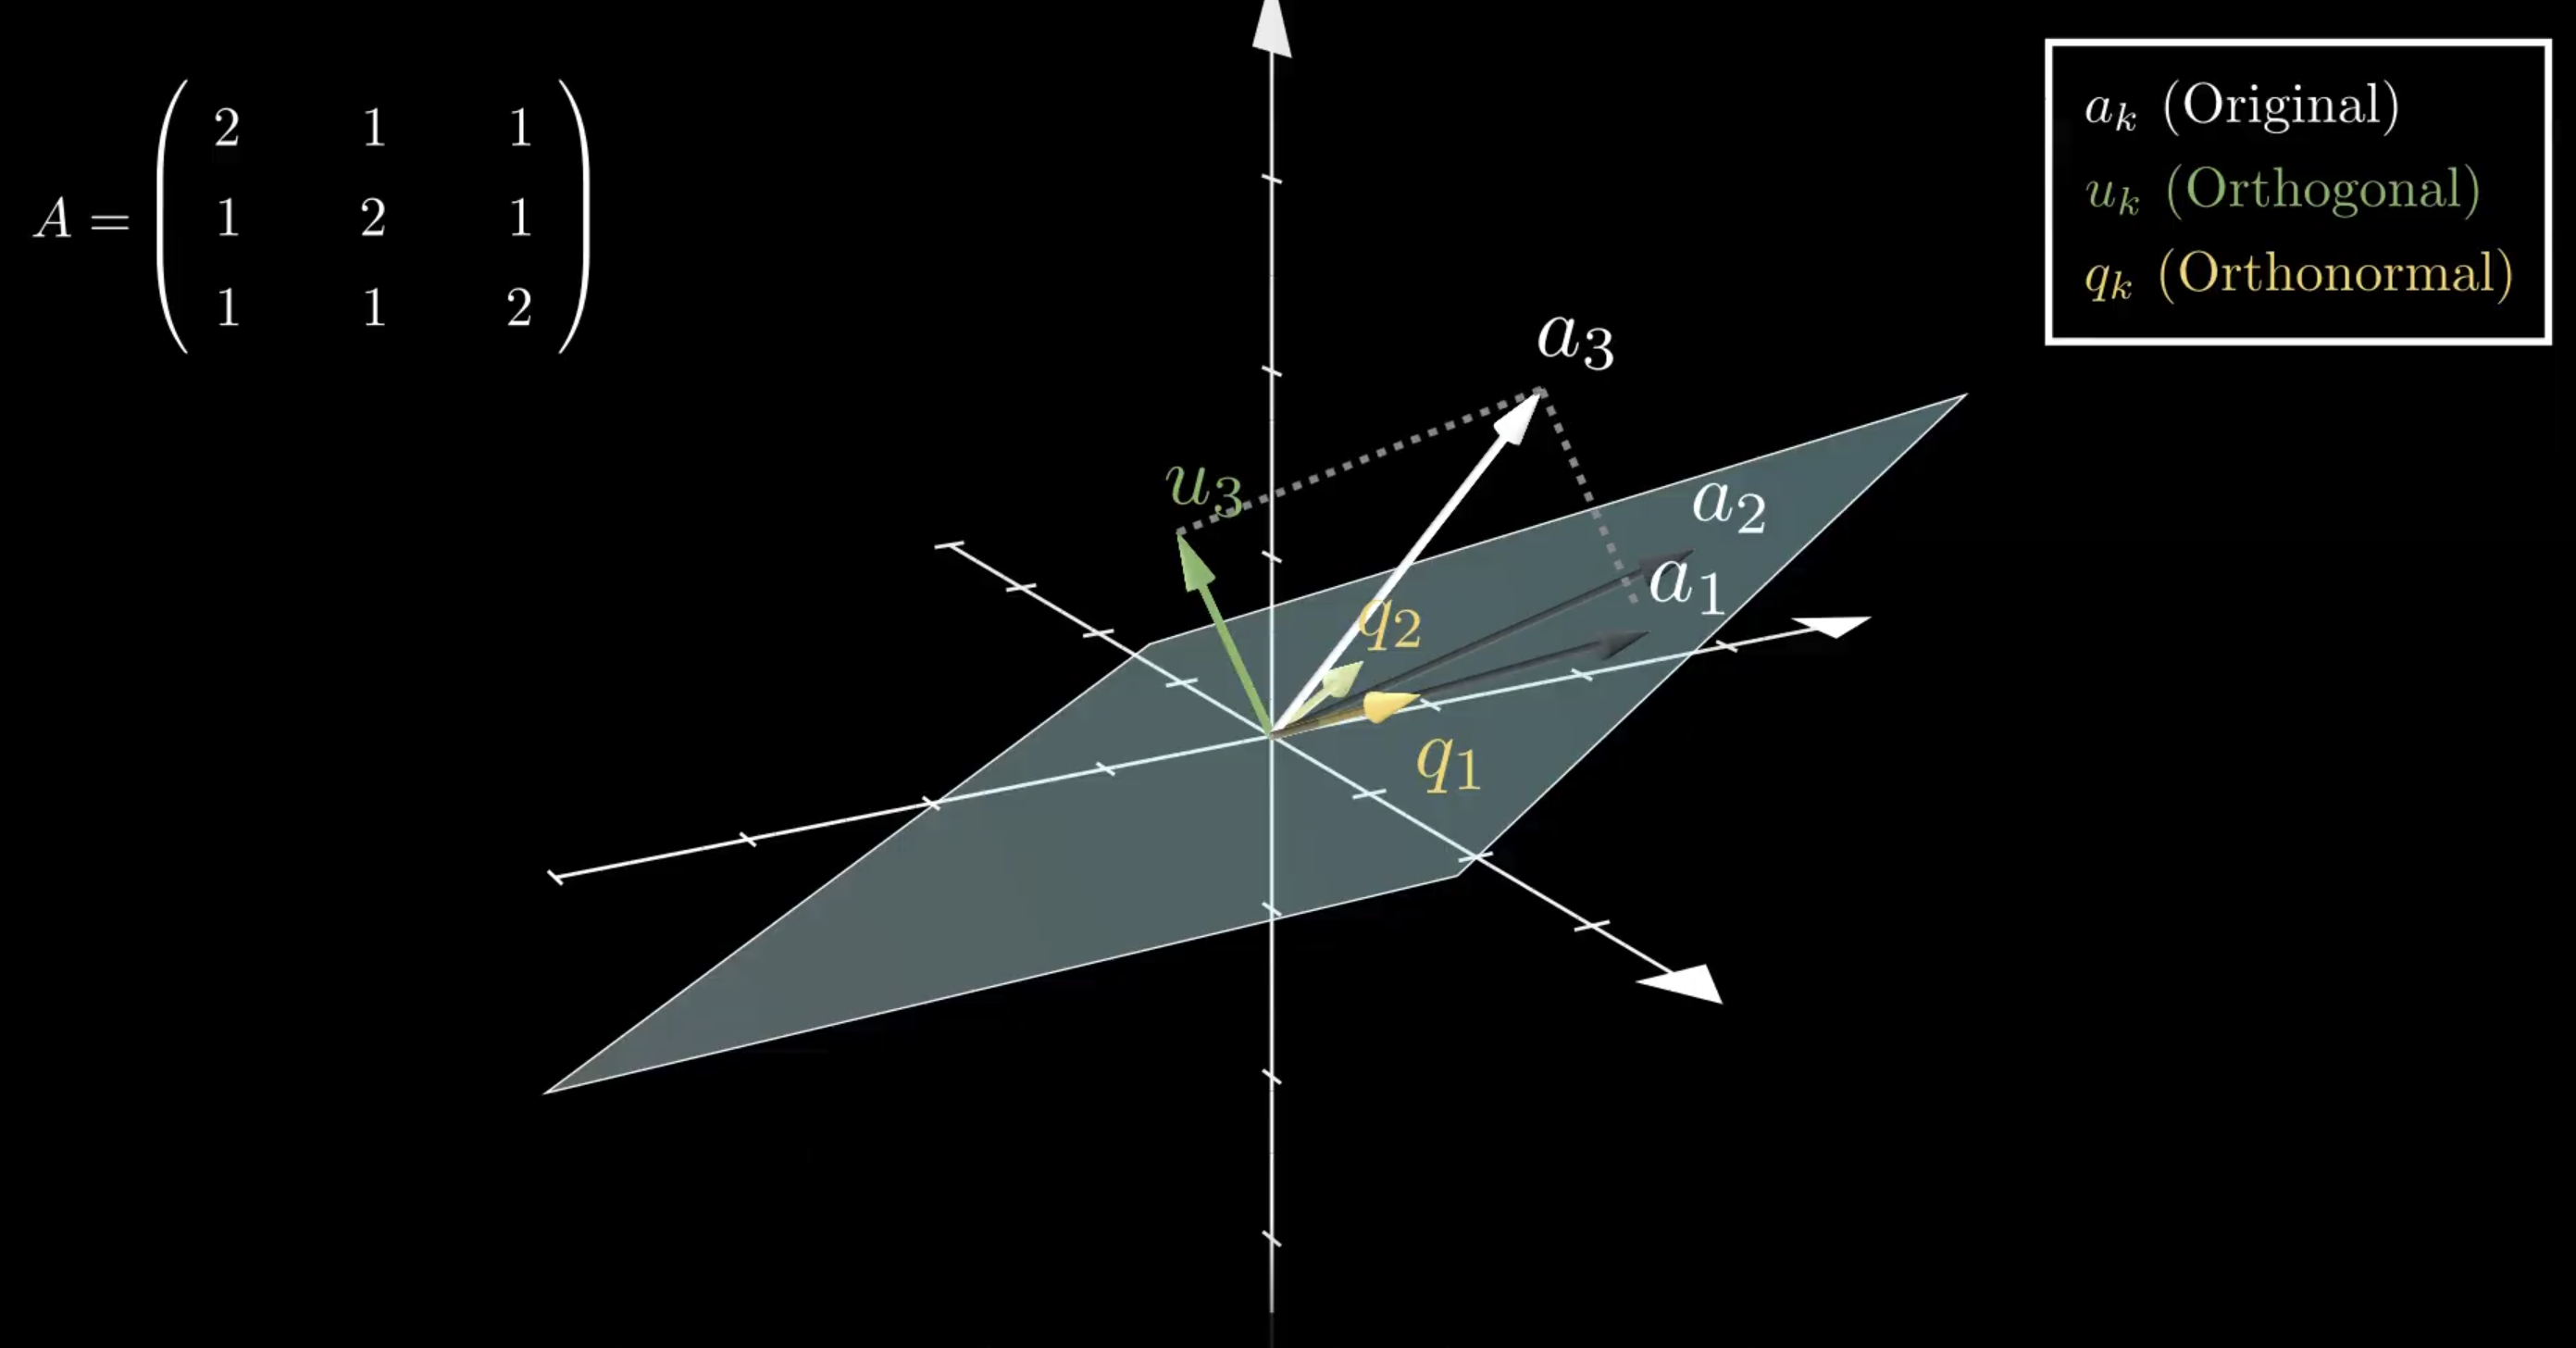
\includegraphics[width=0.7\textwidth]{images/manim1.png}
    \caption{Mô phỏng mặt phẳng không gian con sinh bởi $q_1, q_2$ trong Manim}
\end{figure}

\textbf{Phân cảnh 2: Giải phương trình đặc trưng (Chéo hóa):}
Trình bày các công thức toán học, lần lượt mô phỏng cách giải phương trình đặc trưng $\det(A - \lambda I) = 0$.
Các biểu thức đa thức được khai triển và nhóm lại thành phương trình bậc 3:
$$-(\lambda - 4)(\lambda - 1)^2 = 0$$
Từ đó, trích xuất ra 3 giá trị riêng: $\lambda_1 = 4, \lambda_2 = 1, \lambda_3 = 1$. Sau khi thế ngược vào hệ phương trình, 3 vector riêng độc lập tuyến tính $v_1, v_2, v_3$ lần lượt xuất hiện trên màn hình.

\textbf{Phân cảnh 3: Hình thành ma trận $P$ và $D$:}
Thể hiện mối liên hệ giữa các đại lượng vừa tính toán với công thức chéo hóa $A = PDP^{-1}$. 

Cuối cùng, hiển thị công thức $A = P D P^{-1}$ dưới dạng ma trận tường minh, kết thúc quá trình trực quan hóa.


\begin{figure}[H]
    \centering
    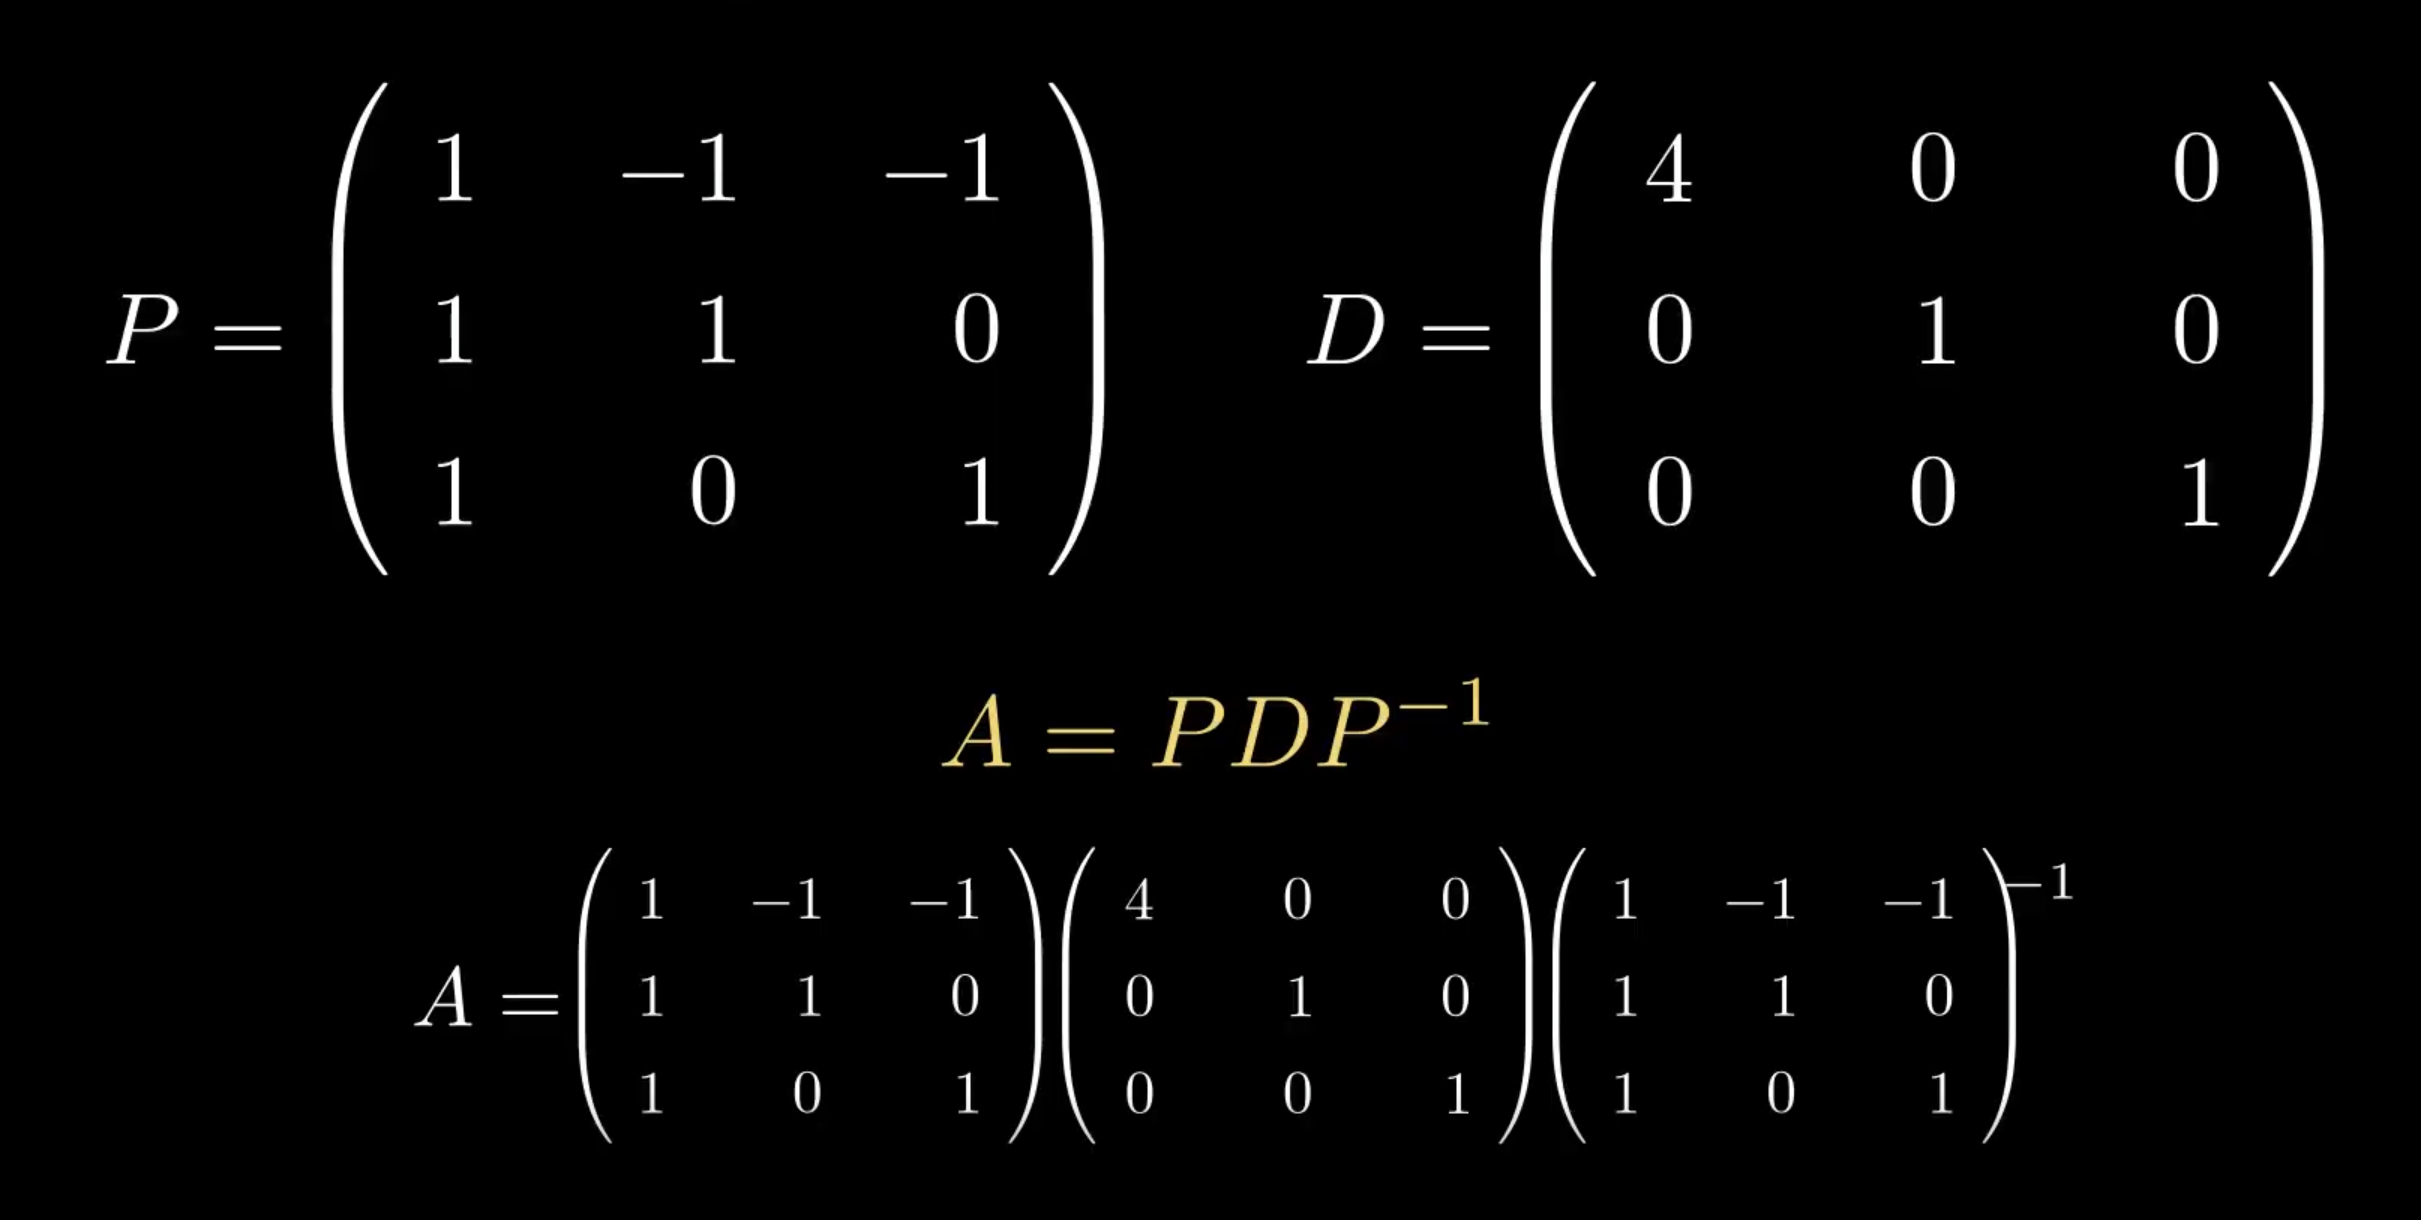
\includegraphics[width=0.7\textwidth]{images/manim2.png}
    \caption{Hiệu ứng chuyển đổi vector riêng thành ma trận $P$ và $D$}
\end{figure}


\subsection*{2.4.2. Ý nghĩa hình học và Ứng dụng thực tế}
\phantomsection
\addcontentsline{toc}{subsection}{2.4.2. Ý nghĩa hình học và Ứng dụng thực tế}

Thông qua video Manim, nhóm đã làm rõ được \textbf{bản chất hình học} của phép chéo hóa đối với ma trận đối xứng. Thay vì coi $A = PDP^{-1}$ là một công thức đại số khô khan, video giúp ta thấy rằng:
\begin{itemize}
    \item Phép nhân ma trận $P^{-1}x$ thực chất là phép đổi hệ tọa độ: chuyển vector $x$ từ hệ cơ sở chuẩn sang hệ tọa độ mới.
    \item Phép nhân với ma trận đường chéo $D$ là một phép co giãn thuần túy dọc theo các trục tọa độ mới này. Chiều của vector riêng tương ứng với $\lambda = 4$ sẽ bị kéo giãn gấp 4 lần, trong khi hai chiều tương ứng với $\lambda = 1$ được giữ nguyên.
    \item Phép nhân với $P$ ở cuối cùng đóng vai trò xoay hệ tọa độ biến dạng đó trở về lại không gian gốc ban đầu.
\end{itemize}

\textbf{Ứng dụng thực tế:}
Việc hiểu rõ cấu trúc $A = PDP^{-1}$ mang lại lợi ích trong thực tế tính toán, cụ thể như:
\begin{enumerate}
    \item \textbf{Tính toán lũy thừa ma trận (Hệ thống động lực):} Việc tìm trạng thái của hệ thống sau $k$ chu kỳ đòi hỏi phải tính $A^k$. Bằng việc chéo hóa, ta dễ dàng thu được $A^k = P D^k P^{-1}$, giảm thiểu hàng triệu phép nhân ma trận thừa thãi xuống chỉ còn việc tính lũy thừa các số trên đường chéo.
    \item \textbf{Phân tích thành phần chính:} Các ma trận hiệp phương sai (Covariance Matrices) trong khoa học dữ liệu luôn là ma trận đối xứng (tương tự ma trận $A$ trong kịch bản video). Việc tìm ra các trị riêng lớn nhất (như $\lambda = 4$) và vector riêng tương ứng giúp các kỹ sư AI giữ lại những đặc trưng quan trọng nhất của tập dữ liệu khổng lồ, đồng thời loại bỏ nhiễu, tạo tiền đề cho các thuật toán nén ảnh và nhận dạng khuôn mặt.
\end{enumerate}
\newpage
\chapter*{\centering{\MakeUppercase{PHẦN 3: THỰC NGHIỆM VÀ PHÂN TÍCH ĐÁNH GIÁ}}}
\phantomsection
\addcontentsline{toc}{chapter}{\textcolor{fitblue}{\MakeUppercase{PHẦN 3: THỰC NGHIỆM VÀ PHÂN TÍCH ĐÁNH GIÁ}}}

\section*{3.1. Giới thiệu tổng quan và Cơ sở lý thuyết}
\phantomsection
\addcontentsline{toc}{section}{3.1. Giới thiệu tổng quan và Cơ sở lý thuyết}

Mục tiêu của phần này là khảo sát, đo lường và đánh giá ba thuật toán giải hệ phương trình tuyến tính $Ax = b$ phổ biến: Khử Gauss, Phân rã QR, và Lặp Gauss-Seidel. Quá trình đánh giá được thực hiện qua hai lăng kính chính: hiệu năng phần mềm (như thời gian thực thi) và tính ổn định số học (sai số làm tròn trên không gian dấu phẩy động).

Theo yêu cầu của đề tài, toàn bộ thuật toán được \textbf{tự lập trình bằng Python thuần} bằng cấu trúc dữ liệu `list of lists` (không sử dụng \texttt{numpy.linalg.solve} hay ma trận `numpy.ndarray` c-extension). Điều này đảm bảo chi phí tính toán lý thuyết và thực tế được phản xạ một cách trung thực nhất.

\textbf{Cơ sở lý thuyết dùng để đánh giá:}
\begin{itemize}
    \item \textbf{Sai số dư tương đối:} Là thước đo độ chính xác của nghiệm tìm được $\hat{x}$ so với vế phải của phương trình bằng chuẩn 2:
    $$ \text{Sai số dư tương đối} = \frac{\|A\hat{x} - b\|_2}{\|b\|_2} $$
    \item \textbf{Độ phức tạp tính toán:} Số phép toán dấu phẩy động (FLOPs). Phân rã trực tiếp (Gauss, QR) đòi hỏi $O(n^3)$ thời gian, trong khi Gauss-Seidel có thể đạt xấp xỉ $O(k n^2)$ nếu hội tụ sau $k$ bước lặp.
    \item \textbf{Số điều kiện và Định lý sai số:} Kí hiệu $\kappa(A) = \|A\| \cdot \|A^{-1}\|$. Đây là đại lượng mô tả mức khuếch đại sai số của hệ phương trình. Định lý sai số cho biết mối quan hệ giữa sai số tương đối của nghiệm (sai số thuận - Forward Error, $\|\Delta x\|/\|x\|$) và sai số tương đối của dữ liệu đầu vào (sai số ngược - Backward Error, $\|\Delta b\|/\|b\|$) qua bất đẳng thức:
    $$ \frac{\|\Delta x\|}{\|x\|} \leq \kappa(A) \cdot \frac{\|\Delta b\|}{\|b\|}. $$
    \item \textbf{Phân rã ma trận lặp:} Với Gauss-Seidel, ta viết $A = D + L + U$ (trong đó $D$ là đường chéo, $L$ là tam giác dưới thuần, $U$ là tam giác trên thuần). Công thức lặp:
    $$ x^{(k+1)} = -(D+L)^{-1}U x^{(k)} + (D+L)^{-1}b. $$
    Dạng theo từng thành phần:
    $$ x_i^{(k+1)} = \frac{1}{a_{ii}}\left(b_i - \sum_{j=1}^{i-1} a_{ij} x_j^{(k+1)} - \sum_{j=i+1}^{n} a_{ij} x_j^{(k)}\right). $$
    Điều kiện hội tụ đủ: ma trận chéo trội chặt theo hàng, tức $|a_{ii}| > \sum_{j \ne i} |a_{ij}|$.
\end{itemize}

\textbf{Bảng so sánh các phương pháp:}
\begin{table}[H]
    \centering
    \caption{So sánh đặc trưng các phương pháp giải hệ tuyến tính}
    \vspace{0.2cm}
    \renewcommand{\arraystretch}{1.2}
    \begin{tabular}{|l|c|l|c|c|}
    \hline
    \textbf{Phương pháp} & \textbf{Loại} & \textbf{Điều kiện áp dụng} & \textbf{Chi phí} & \textbf{Ổn định} \\ \hline
    Gauss (Partial Pivoting) & Trực tiếp & Mọi $A$ khả nghịch & $O(n^3)$ & Cao \\ \hline
    QR (Gram-Schmidt) & Trực tiếp & Mọi $A$ (kể cả chữ nhật) & $O(n^3)$ & Rất cao \\ \hline
    Gauss--Seidel & Lặp & Chéo trội hàng / SPD & $O(k n^2)$ & Trung bình \\ \hline
    \end{tabular}
\end{table}

\section*{3.2. Cài đặt thuật toán giải hệ phương trình tuyến tính}
\phantomsection
\addcontentsline{toc}{section}{3.2. Cài đặt thuật toán giải hệ phương trình tuyến tính}

Khối mã giả dưới đây chi tiết hóa quy trình thực thi của 3 thuật toán nền tảng. Các thuật toán được thiết kế để xử lý dữ liệu đầu vào là ma trận vuông $A$ và vector $b$, trả về nghiệm tối ưu $x$ tiệm cận với nghiệm thực tế của hệ phương trình.

\subsection*{3.2.1. Phương pháp Khử Gauss (Partial Pivoting)}
\phantomsection
\addcontentsline{toc}{subsection}{3.2.1. Phương pháp Khử Gauss (Partial Pivoting)}

Thuật toán khử Gauss là phương pháp trực tiếp, bản chất biến đổi hệ phương trình gốc về dạng tam giác trên để giải bằng thế ngược. Việc áp dụng cơ chế Partial Pivoting (chọn phần tử chốt lớn nhất theo trị tuyệt đối trên cột khử hiện tại, rồi hoán vị hàng) là bắt buộc để đảm bảo tính ổn định số học.

\begin{algorithm}[H]
\caption{Giải hệ phương trình bằng Khử Gauss (Partial Pivoting)}
\label{alg:gauss_pivoting}
\begin{algorithmic}[1]
\Procedure{SOLVE\_GAUSS}{$A, b$}
    \State $n \gets \text{size}(A)$
    \For{$i \gets 0$ to $n-1$}
        \State $max\_row \gets i$; $max\_val \gets |A[i][i]|$
        \For{$k \gets i+1$ to $n-1$} \Comment{Tìm phần tử chốt lớn nhất}
            \If{$|A[k][i]| > max\_val$}
                \State $max\_val \gets |A[k][i]|$; $max\_row \gets k$
            \EndIf
        \EndFor
        \State Hoán vị hàng $i$ và $max\_row$ cho cả $A$ và $b$
        \For{$k \gets i+1$ to $n-1$} \Comment{Khử các dòng phía dưới}
            \State $factor \gets A[k][i] / A[i][i]$
            \For{$j \gets i+1$ to $n-1$}
                \State $A[k][j] \gets A[k][j] - factor \times A[i][j]$
            \EndFor
            \State $b[k] \gets b[k] - factor \times b[i]$
        \EndFor
    \EndFor
    \State $x \gets$ giải bằng thế ngược từ $A$ và $b$ đã khử tam giác
    \State \Return $x$
\EndProcedure
\end{algorithmic}
\end{algorithm}

\subsection*{3.2.2. Phương pháp Phân rã QR (Gram-Schmidt)}
\phantomsection
\addcontentsline{toc}{subsection}{3.2.2. Phương pháp Phân rã QR (Gram-Schmidt)}

Ứng dụng thuật toán trực giao hóa Gram-Schmidt để phân rã ma trận gốc thành tích $A = QR$ (với $Q$ là ma trận trực giao và $R$ là ma trận tam giác trên). So với Gauss phụ thuộc vào pivoting, hướng tiếp cận QR ổn định hơn, đặc biệt đối với các ma trận có số điều kiện lớn. Bài toán được giải thông qua hệ trung gian $Rx = Q^Tb$.

\begin{algorithm}[H]
\caption{Giải hệ phương trình bằng Phân rã QR (Gram-Schmidt)}
\label{alg:solve_qr}
\begin{algorithmic}[1]
\Procedure{SOLVE\_QR}{$A, b$}
    \State $n \gets \text{size}(A)$
    \State $Q, R \gets \text{Ma trận không } n \times n$
    \For{$j \gets 0$ to $n-1$} \Comment{Quy trình Gram-Schmidt cải tiến}
        \State $v \gets A[0 \dots n-1][j]$
        \For{$i \gets 0$ to $j-1$}
            \State $R[i][j] \gets \sum_{k=0}^{n-1} Q[k][i] \times v[k]$
            \State $v \gets v - R[i][j] \times Q[0 \dots n-1][i]$
        \EndFor
        \State $R[j][j] \gets \|v\|_2$
        \State $Q[0 \dots n-1][j] \gets v / R[j][j]$
    \EndFor
    \State $y \gets Q^T b$
    \State $x \gets$ giải thế ngược từ $Rx = y$
    \State \Return $x$
\EndProcedure
\end{algorithmic}
\end{algorithm}

\subsection*{3.2.3. Phương pháp Lặp Gauss-Seidel}
\phantomsection
\addcontentsline{toc}{subsection}{3.2.3. Phương pháp Lặp Gauss-Seidel}

Trái với hai phương pháp trực tiếp, Gauss-Seidel là thuật toán lặp: bắt đầu với một đoán trước ban đầu $x^{(0)} = \vec{0}$, thuật toán thay thế nghiệm mới tức thời vào bên trong mô hình để sinh ra nghiệm hội tụ. Phương pháp này chỉ thành công khi ma trận đạt tính chất đường chéo trội nghiêm ngặt hoặc đối xứng xác định dương.

\begin{algorithm}[H]
\caption{Giải hệ phương trình bằng Lặp Gauss-Seidel}
\label{alg:gauss_seidel}
\begin{algorithmic}[1]
\Procedure{GAUSS\_SEIDEL}{$A, b, max\_iters, tol$}
    \State $x \gets$ mảng $n$ phần tử 0; $n \gets$ cấp của $A$
    \For{$it \gets 1$ to $max\_iters$}
        \State $max\_diff \gets 0$
        \For{$i \gets 0$ to $n-1$}
            \State $s \gets \sum_{j \neq i} A[i][j] \times x[j]$
            \State $x_{new} \gets (b[i] - s) / A[i][i]$
            \State $max\_diff \gets \max(max\_diff, |x_{new} - x[i]|)$
            \State $x[i] \gets x_{new}$
        \EndFor
        \If{$max\_diff < tol$}
            \State \textbf{break} \Comment{Hội tụ}
        \EndIf
    \EndFor
    \State \Return $x$
\EndProcedure
\end{algorithmic}
\end{algorithm}

\section*{3.3. Thực nghiệm đo lường hiệu năng và phân tích}
\phantomsection
\addcontentsline{toc}{section}{3.3. Thực nghiệm đo lường hiệu năng và phân tích}

Để đánh giá độ phức tạp thời gian theo kích thước bài toán, nhóm sinh ngẫu nhiên các ma trận vuông chéo trội nghiêm ngặt nhằm đảm bảo hội tụ của Gauss--Seidel. Tập kích thước thử nghiệm là $n \in \{50, 100, 200, 500, 1000\}$. Thời gian được đo bằng \texttt{time.perf\_counter()}; với $n < 500$ chạy $5$ lần lấy trung bình, với $n = 500, 1000$ chạy $1$ lần để tránh thời gian quá dài.

\textbf{Bảng thống kê kết quả chạy thực nghiệm (trích xuất từ cấu hình đo lường Notebook):}
\begin{table}[H]
    \centering
    \caption{So sánh thời gian chạy thực tế (s) và sai số dư tương đối theo các hệ $N$}
    \vspace{0.2cm}
    \renewcommand{\arraystretch}{1.3}
    \resizebox{\textwidth}{!}{
        \begin{tabular}{|c|c|c|c|c|c|c|}
        \hline
        \textbf{Cấp $n$} & \textbf{Khử Gauss Time} & \textbf{Sai số dư Gauss} & \textbf{QR Time} & \textbf{Sai số dư QR} & \textbf{G-Seidel Time} & \textbf{Sai số dư GS} \\ \hline
        50   & 0.002820 s & $1.90 \times 10^{-16}$ & 0.010590 s & $1.24 \times 10^{-16}$ & \textbf{0.002894 s} & $4.84 \times 10^{-11}$ \\ \hline
        100  & 0.020056 s & $2.97 \times 10^{-16}$ & 0.079861 s & $1.39 \times 10^{-16}$ & \textbf{0.011074 s} & $7.17 \times 10^{-11}$ \\ \hline
        200  & 0.159520 s & $3.69 \times 10^{-16}$ & 0.856179 s & $1.89 \times 10^{-16}$ & \textbf{0.045281 s} & $5.60 \times 10^{-11}$ \\ \hline
        500  & 2.971386 s & $6.67 \times 10^{-16}$ & 12.450867 s & $2.58 \times 10^{-16}$ & \textbf{0.295427 s} & $7.12 \times 10^{-11}$ \\ \hline
        1000 & 27.374951 s & $9.95 \times 10^{-16}$ & 111.553300 s & $3.18 \times 10^{-16}$ & \textbf{1.256143 s} & $8.07 \times 10^{-11}$ \\ \hline
        \end{tabular}
    }
\end{table}

\begin{figure}[H]
    \centering
    % Lưu ảnh log_log_plot.png vào folder images
    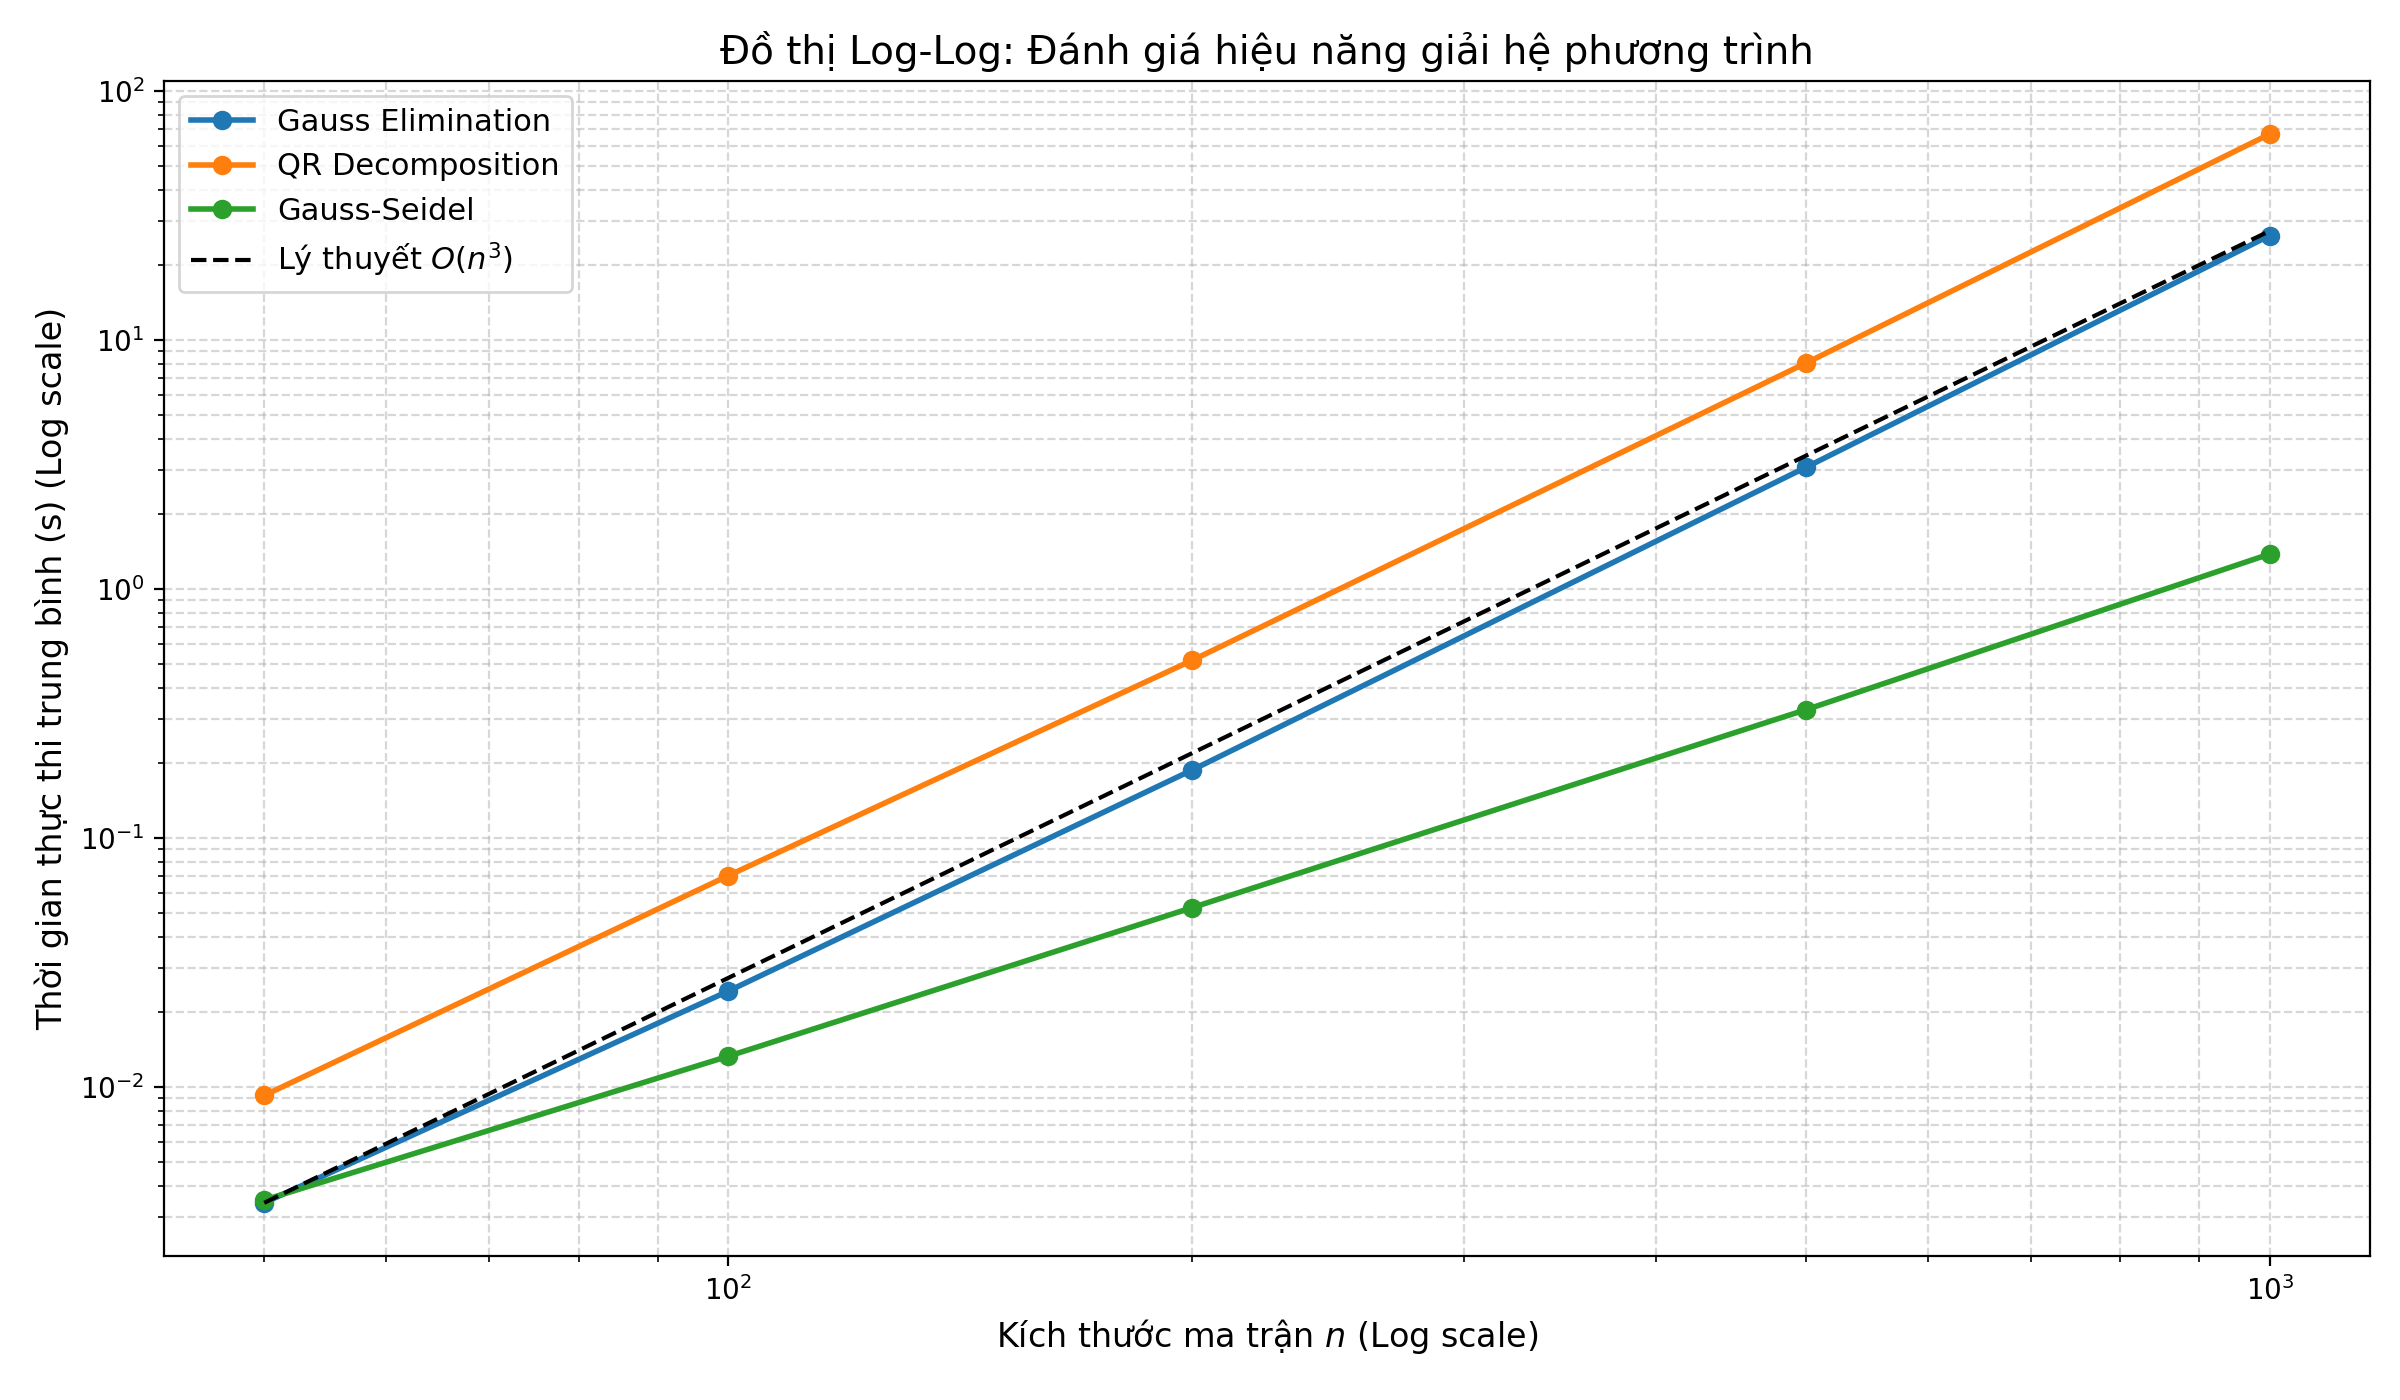
\includegraphics[width=0.8\textwidth]{images/log_log_plot.png}
    \caption{Đồ thị Log-Log mô phỏng trực quan thời gian chạy của ba phương pháp}
\end{figure}

Việc vẽ đồ thị theo nguyên lý Logarit cơ số kép (Log-Log plot) biến các đường cong đa thức $T(n) = c \cdot n^\alpha$ thành các đường thẳng có hệ số góc bằng hệ số mũ $\alpha$, giúp ta dễ dàng tính được bậc độ phức tạp lý thuyết thực tế. Từ đồ thị trên và các số liệu thuộc bảng kiểm nghiệm, ta trực tiếp rút ra ba nhóm kết luận khoa học vững chắc:

\subsection*{3.3.1. Phân tích Khử Gauss (Partial Pivoting)}
Đường đo lường trên không gian log-log bám sát lý thuyết $O(n^3)$ (hệ số góc $\alpha \approx 3$). Phương pháp mất khoảng $27.37$ giây để giải hệ $n=1000$, đồng thời duy trì sai số dư tương đối quanh mức $10^{-16}$, tiệm cận giới hạn máy chính xác (machine epsilon) của float64. Kỹ thuật partial pivoting giúp ổn định quá trình khử và tránh chia cho phần tử chốt quá nhỏ.

\subsection*{3.3.2. Phân tích Phân rã QR (Gram-Schmidt)}
Mặc dù có cùng hệ số góc $\alpha \approx 3$, thời gian thực thi của QR luôn cao hơn Gauss. Ở $n=1000$, QR tốn $111.55$ giây, lớn hơn khoảng $4.07$ lần so với Gauss. Lý do đến từ chi phí trực giao hóa trong Gram-Schmidt, vốn có hằng số lớn hơn trong $O(n^3)$. Đổi lại, QR ổn định hơn khi ma trận gần suy biến.

\subsection*{3.3.3. Hiệu năng của phương pháp lặp Gauss-Seidel}
Đường Gauss--Seidel có độ dốc nhỏ hơn so với hai phương pháp trực tiếp. Với $n=1000$, thời gian là $1.26$ giây. Kết quả này đến từ việc mỗi vòng lặp chỉ tốn $O(n^2)$ phép tính; khi ma trận chéo trội nghiêm ngặt, số vòng lặp hội tụ $k$ không quá lớn, dẫn đến chi phí tổng quát $O(k n^2)$.

\subsection*{3.3.4. Phân tích chi phí tính toán và Truy xuất Bộ nhớ}
Việc phân giải cơ chế thời gian thực thi của các phương pháp trên không chỉ dựa vào mô hình Toán lý thuyết mà còn phụ thuộc vào kiến trúc phần cứng máy tính. Về chi phí tính toán (FLOPs), thuật toán Gauss cơ bản yêu cầu xấp xỉ $\frac{2}{3}n^3$ phép nhân-cộng dấu phẩy động; trong khi kịch bản trực giao hóa của thuật giải Gram-Schmidt (QR) tiến hành $\approx 2n^3$ thao tác liên kết tổng vector và bình phương Euclidean. 

Thực tế ghi nhận sự chênh lệch thời gian ở $N=1000$ là $(111.55/27.37) \approx 4.07$ lần. Sự khác biệt này đến từ chi phí trực giao hóa trong QR và cách truy xuất bộ nhớ. Với \texttt{list of lists}, truy xuất theo cột trong QR kém liên tục hơn so với truy xuất theo hàng trong Gauss, làm tăng độ trễ truy xuất bộ nhớ.
\section*{3.4. Phân tích tính ổn định số học: Ma trận Hilbert vs. SPD}
\phantomsection
\addcontentsline{toc}{section}{3.4. Phân tích tính ổn định số học: Ma trận Hilbert vs. SPD}

Độ chính xác của hệ phương trình $Ax = b$ không chỉ phụ thuộc vào cơ chế thuật toán, mà còn vấp vào đặc thù cấu trúc toán học của bản thân ma trận $A$. Phép đánh giá này được thực hiện để chứng minh vấn đề về sai số do hiện tượng làm tròn (round-off error) đối với các hệ thống có tính đa cộng tuyến cao – được đánh giá thông qua chỉ số của Số điều kiện $\kappa(A)$.

\subsection*{3.4.1. Thiết lập biến cố thực nghiệm}
Nhóm đối chiếu sai số dư của hai dạng ma trận vuông với kích thước cơ sở $n=10$:
\begin{itemize}
    \item \textbf{Ma trận Hilbert ($H_n$):} Khởi tạo dưới dạng $H_{ij} = \frac{1}{i+j-1}$. Ma trận này được biết đến với cấu trúc đặc trưng thiếu điều kiện số học hay hệ điều kiện kém (ill-conditioned) do khoảng cách giữa các vector cột vô cùng gần nhau.
    \item \textbf{Ma trận Đối xứng Xác Định Dương (SPD):} Khởi tạo bằng phép nhân $A = X^T X + nI$ để bảo đảm tính xác định dương.
\end{itemize}
Đối với Gauss--Seidel, điều kiện hội tụ đủ là chéo trội; tuy nhiên với ma trận SPD, phương pháp vẫn hội tụ theo lý thuyết, dù không nhất thiết thỏa chéo trội theo hàng.
Trong thí nghiệm này, số điều kiện được trình bày theo $\kappa(A)$ như trong notebook thực nghiệm.

\begin{table}[H]
    \centering
    \caption{Sai số dư và số điều kiện (chuẩn vô cùng) với $N=10$}
    \vspace{0.2cm}
    \renewcommand{\arraystretch}{1.3}
    \begin{tabular}{|c|c|c|c|c|}
    \hline
    \textbf{Loại ma trận} & \textbf{Số điều kiện $\kappa(A)$} & \textbf{Sai số dư Gauss} & \textbf{Sai số dư QR} & \textbf{Sai số dư GS} \\ \hline
    Hilbert (Ill-conditioned) & $1.60 \times 10^{13}$ & $0.00$ & $2.20 \times 10^{-6}$ & $4.19 \times 10^{-6}$ \\ \hline
    SPD (Well-conditioned) & $2.20$ & $1.96 \times 10^{-16}$ & $2.10 \times 10^{-16}$ & $1.22 \times 10^{-11}$ \\ \hline
    \end{tabular}
\end{table}

\begin{figure}[H]
    \centering
    % Lưu ảnh condition_number_plot.png từ IPython Jupyter Data
    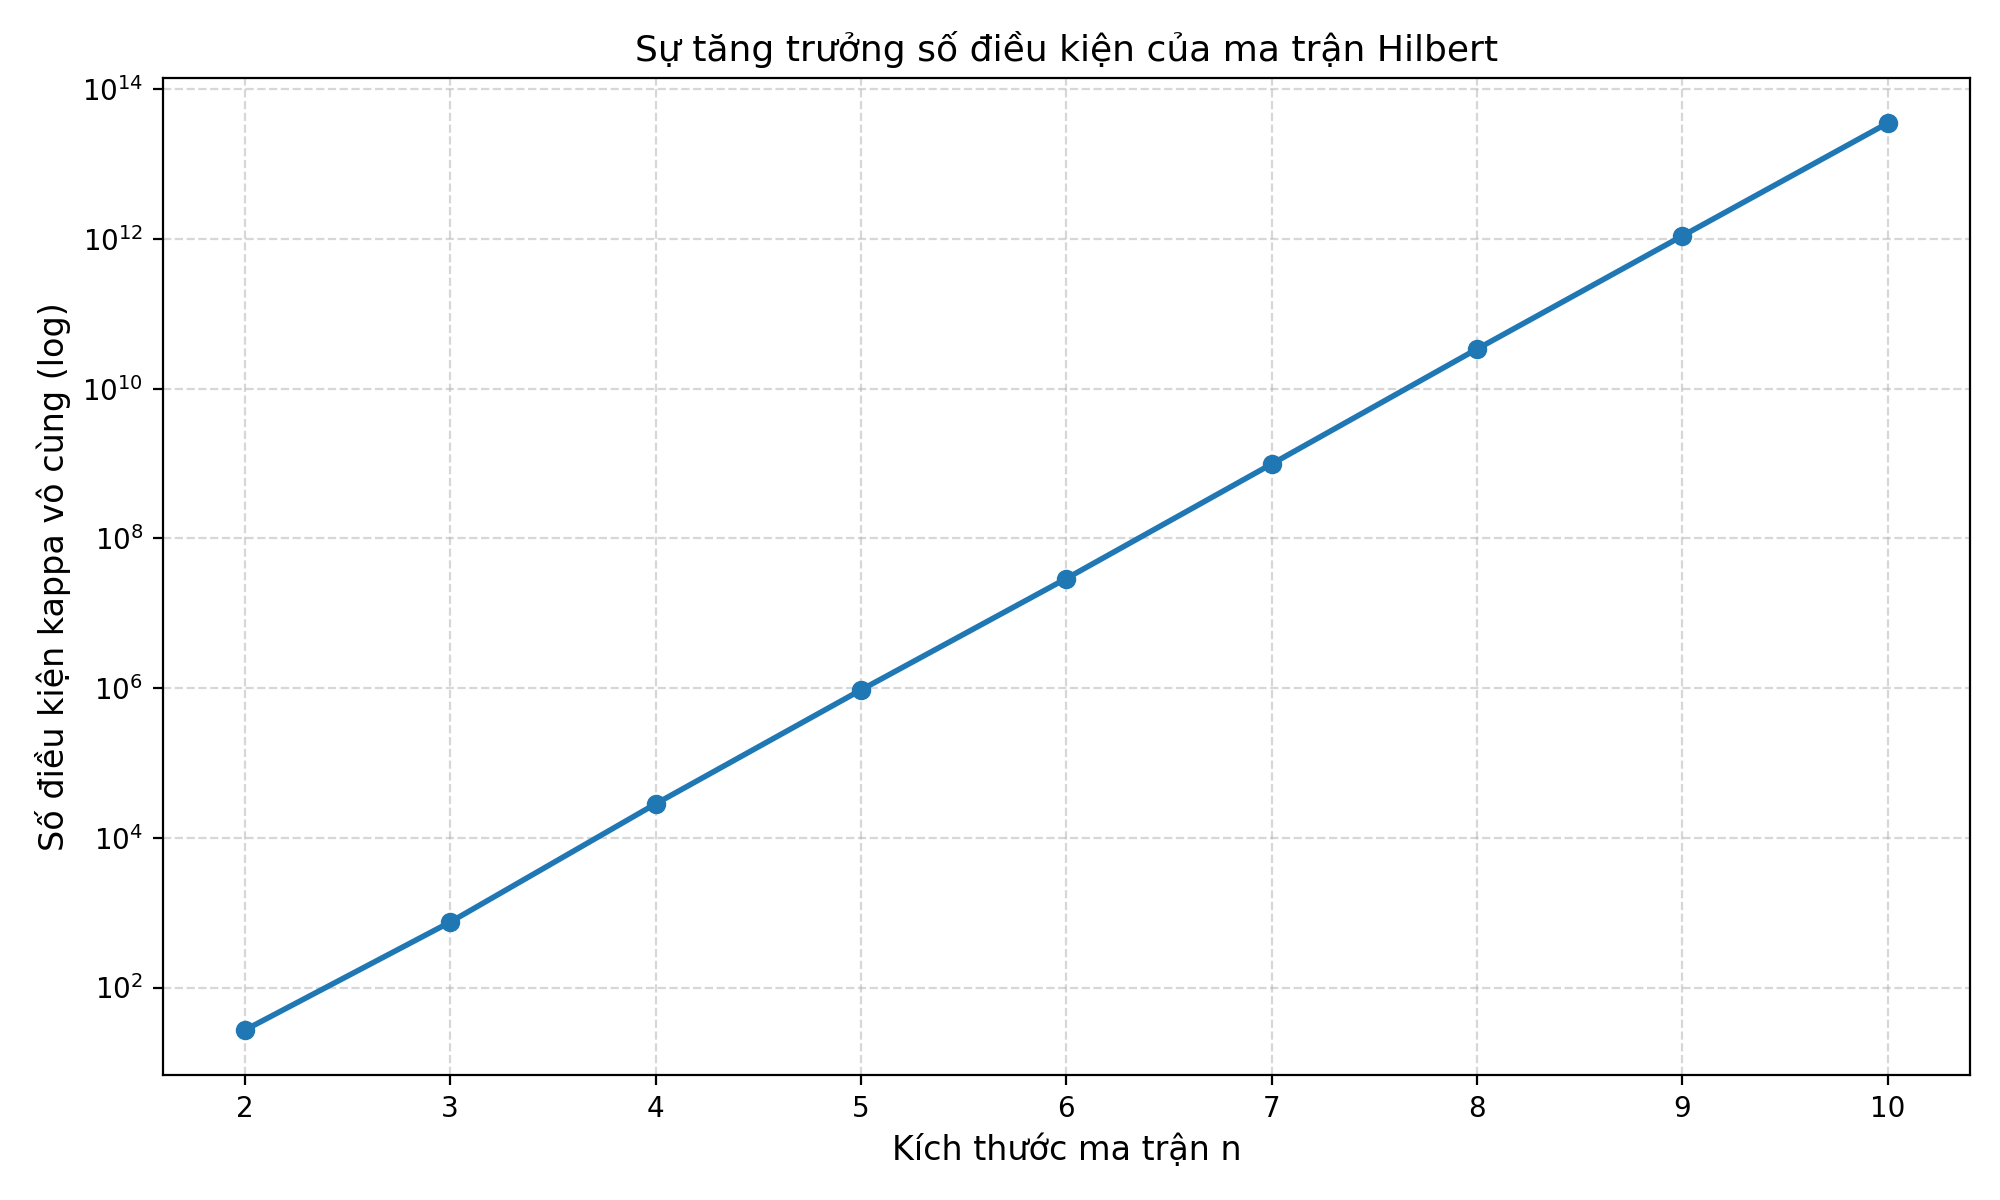
\includegraphics[width=0.8\textwidth]{images/condition_number_plot.png}
    \caption{Biểu đồ phân tích độ khuếch đại của số điều kiện Hilbert khi kích thước ma trận n gia tăng}
\end{figure}

\subsection*{3.4.2. Phân tích sai số theo số điều kiện}
Ma trận Hilbert có $\kappa(A)$ rất lớn ($\approx 1.6 \times 10^{13}$), dẫn đến sai số dư của QR và Gauss--Seidel ở mức $10^{-6}$. Trong khi đó, ma trận SPD có $\kappa(A)$ nhỏ ($\approx 2.2$), nên cả Gauss và QR đều đạt sai số dư gần $10^{-16}$. Kết quả này phù hợp với lý thuyết sai số: khi $\kappa(A)$ lớn, sai số bị khuếch đại đáng kể ngay cả khi thuật toán ổn định.

Ở trường hợp SPD, Gauss--Seidel vẫn cho sai số dư lớn hơn hai phương pháp trực tiếp. Nguyên nhân chính là đây là phương pháp lặp với ngưỡng dừng hữu hạn, nên sai số dư không thể tiệm cận máy chính xác như Gauss và QR.

\subsection*{3.4.3. Kết luận về tính ổn định của thuật toán}
Kết quả thực nghiệm cho thấy việc \textbf{kiểm định số điều kiện} là bước bắt buộc trước khi giải hệ tuyến tính. Các ma trận ill-conditioned như Hilbert có thể làm mất độ tin cậy của nghiệm ngay cả với kích thước nhỏ. Điều này khẳng định rằng tối ưu hóa mã nguồn không thể thay thế cho việc đánh giá điều kiện của bài toán.

\section*{3.5. Chỉ dẫn lựa chọn giải thuật}
Dựa trên sự cân bằng giữa chi phí thực thi và độ ổn định số học, nhóm đề xuất quy trình lựa chọn thuật toán giải hệ $Ax = b$ như sau:

\begin{itemize}
    \item \textbf{Phương pháp Khử (Gauss / LU / Cholesky):} Ưu tiên sử dụng cho các ma trận đặc (Dense Matrices) có kích thước từ nhỏ đến trung bình (dưới 10.000 ẩn số) và có số điều kiện thấp ($\kappa(A) < 10^3$). Đây là lựa chọn tối ưu về mặt tốc độ trong điều kiện ma trận ổn định.
    \item \textbf{Phương pháp Trực giao (QR):} Áp dụng cho các bài toán yêu cầu độ ổn định số học cao hoặc các hệ phương trình không vuông (mô hình hồi quy, Bình phương tối thiểu). Mặc dù chi phí thời gian cao hơn, QR đảm bảo tính chính xác cho các hệ có nguy cơ nhiễu số học.
    \item \textbf{Phương pháp Lặp (Gauss-Seidel):} Là lựa chọn hàng đầu cho các ma trận thưa quy mô lớn (Sparse Matrices với tỷ lệ phần tử khác 0 thấp), ma trận đường chéo trội hoặc các hệ phương trình đạo hàm riêng (PDEs). Phương pháp này tối ưu hóa việc sử dụng bộ nhớ và thời gian tính toán thông qua cơ chế hội tụ dần.
\end{itemize}

\newpage
\chapter*{\centering{\MakeUppercase{Kết luận}}}
\phantomsection
\addcontentsline{toc}{chapter}{\textcolor{fitblue}{\MakeUppercase{Kết luận}}}

\section*{1. Các kết quả đạt được}
\phantomsection
\addcontentsline{toc}{section}{1. Các kết quả đạt được}
Sau quá trình nghiên cứu, thiết kế thuật toán và lập trình thực nghiệm, nhóm đã hoàn thành các mục tiêu đề ra của Đồ án môn Toán Ứng dụng và Thống kê. Cụ thể:
\begin{itemize}
    \item \textbf{Về mặt Lập trình \& Thuật toán:} Cài đặt thành công các hàm từ đầu bằng Python thuần. Cài đặt thuật toán Khử Gauss có chọn phần tử chốt (Partial Pivoting) giúp đảm bảo độ chính xác cao khi giải hệ phương trình và tìm nghịch đảo. Tại phần phân rã, nhóm đã triển khai thành công thuật toán trực giao hóa Gram-Schmidt cổ điển và thuật toán Lặp QR (QR Iteration) để tìm giá trị riêng, vector riêng và chéo hóa ma trận.
    \item \textbf{Về mặt Đánh giá \& Kiểm thử:} Xây dựng được hệ thống testcase bao phủ các trường hợp từ ma trận lý tưởng, ma trận suy biến, đến các ma trận số học như ma trận Hilbert hay ma trận chênh lệch tỷ lệ cực đoan (Extreme Scale).
    \item \textbf{Về mặt Trực quan hóa:} Render thành công video 3D bằng Manim mô phỏng trực quan từng bước chiếu vector của thuật toán Gram-Schmidt và hiệu ứng tạo lập không gian tọa độ mới trong phép biến đổi $A = PDP^{-1}$.
\end{itemize}

\section*{2. Khó khăn gặp phải}
\phantomsection
\addcontentsline{toc}{section}{2. Khó khăn gặp phải}
Trong quá trình thực hiện đồ án, nhóm đã đối mặt và giải quyết nhiều thách thức khó khăn, đặc biệt là ở mảng Tính toán số (Numerical Computing):
\begin{itemize}
    \item \textbf{Sai số làm tròn (Round-off Errors) trong Gram-Schmidt:} Thuật toán Gram-Schmidt cổ điển thể hiện sự bất ổn định số học nghiêm trọng khi gặp các vector gần phụ thuộc tuyến tính (Numerically Dependent). Hiện tượng triệt tiêu sai số (Catastrophic Cancellation) khiến ma trận $Q$ nhanh chóng mất đi tính trực giao hoàn hảo.
    \item \textbf{Tốc độ hội tụ của thuật toán Lặp QR:} Do giới hạn yêu cầu tự cài đặt, thuật toán Lặp QR thuần túy (không có cơ chế dịch chuyển Shifts) mất rất nhiều thời gian (hàng trăm vòng lặp) mới có thể hội tụ khi gặp các trị riêng nằm quá sát nhau. 
    \item \textbf{Trực quan hóa không gian 3D:} Thư viện Manim có learning-curve (đường cong học tập) khá dốc. Việc đồng bộ hóa các phép chiếu toán học với hoạt ảnh (animations) của camera 3D tốn rất nhiều thời gian canh chỉnh tọa độ.
    \item \textbf{Kiến thức khó:} Đồ án có nhiều phần kiến thức khó, đòi hỏi phải nghiên cứu nhiều tài liệu tham khảo và tham khảo nhiều nguồn trên Internet, khó khăn nhất là cài các thuật toán mà không sử dụng thư viện Numpy.
\end{itemize}

\section*{3. Bài học rút ra}
\phantomsection
\addcontentsline{toc}{section}{3. Bài học rút ra}
Sau quá trình cùng nhau hoàn thành đồ án thì nhóm có rút ra được một số bài học cho mình:
\begin{enumerate}
    \item \textbf{Khoảng cách giữa lý thuyết và thực hành:} Một công thức toán học đúng hoàn toàn trên giấy (như Gram-Schmidt) chưa chắc đã là một thuật toán tốt khi đưa vào bộ nhớ dấu phẩy động (Float 64-bit) của máy tính. Việc hiểu rõ giới hạn phần cứng giúp nhóm có tư duy lập trình phòng thủ tốt hơn.
    \item \textbf{Hiểu sâu hơn về các thư viện công nghiệp:} Qua việc tự cài đặt và liên tục nhận kết quả thua kém so với NumPy ở các test cases khó, nhóm đã hiểu được tại sao các thư viện hiện đại phải sử dụng những thuật toán phức tạp hơn rất nhiều như Householder Reflections (để phân rã) và Wilkinson Shifts (để chéo hóa).
    \item \textbf{Kỹ năng:} Qua quá trình cùng nhau làm và nghiên cứu các tài liệu, từng thành viên trong nhóm đồng thời phát triển nhiều kĩ năng mềm như: research, làm việc nhóm, giao tiếp. Các kĩ năng trên đều là kỹ năng nền tảng quan trọng cho tương lai sau này.
\end{enumerate}
\newpage
\phantomsection
\addcontentsline{toc}{chapter}{\textcolor{fitblue}{\MakeUppercase{Tài liệu tham khảo}}}
\nocite{*} % Ép hiển thị toàn bộ tài liệu trong file .bib dù không có lệnh \cite
\printbibliography[title={TÀI LIỆU THAM KHẢO}]
\newpage
% --- CHƯƠNG PHỤ LỤC DUY NHẤT ---
\setcounter{chapter}{4} % Giữ chapter counter để đồng bộ hệ thống nếu cần
\chapter*{\centering{\MakeUppercase{Phụ lục}}}
\phantomsection
\addcontentsline{toc}{chapter}{\textcolor{fitblue}{PHỤ LỤC}}

% --- MỤC: DANH MỤC HÌNH ẢNH ---
\section*{Danh mục Hình ảnh}
\phantomsection
\addcontentsline{toc}{section}{Danh mục Hình ảnh}
\makeatletter
\vspace{-0.5cm} 
\@starttoc{lof}
\makeatother

% --- MỤC: DANH MỤC BẢNG BIỂU ---
\section*{Danh mục Bảng biểu}
\phantomsection
\addcontentsline{toc}{section}{Danh mục Bảng biểu}
\makeatletter
\vspace{-0.5cm}
\@starttoc{lot}
\makeatother

% --- MỤC: DANH MỤC MÃ GIẢ ---
\section*{Danh mục Mã giả}
\phantomsection
\addcontentsline{toc}{section}{Danh mục Mã giả}
\makeatletter
\providecommand*{\l@algorithm}{\@dottedtocline{1}{1.5em}{2.3em}}
\vspace{-0.5cm}
\@starttoc{loa}
\makeatother

% --- MỤC: TÀI NGUYÊN VÀ ĐƯỜNG DẪN ---
\section*{Tài nguyên và Đường dẫn}
\phantomsection
\addcontentsline{toc}{section}{Tài nguyên và Đường dẫn}

\begin{itemize}
    \item \textbf{Video Demo (Manim):} \url{https://drive.google.com/file/d/1I-pOLFwKOWMM5jLq7blxnKZRxq0EeHbf/view?usp=sharing}
    \item \textbf{Kho lưu trữ GitHub:} \url{https://github.com/anhtuan0806/Matrices_and_Foundations_of_Scientific_Computing}
\end{itemize}



\end{document}